\documentclass[journal]{IEEEtran}
\usepackage{times}

% numbers option provides compact numerical references in the text. 

\usepackage{graphics} % for pdf, bitmapped graphics files
\usepackage{epsfig} % for postscript graphics files
%\usepackage{mathptmx}
%\usepackage{newtxtext}
%\usepackage{newtxmath}
\usepackage{times} % assumes new font selection scheme installed
\usepackage{amsmath} % assumes amsmath package installed
\usepackage{amssymb}  % assumes amsmath package installed
\usepackage{amsthm}
\usepackage{mathtools}
\usepackage{bm}
\usepackage{mathrsfs}
\usepackage{xcolor}
\usepackage{cite}
\usepackage{threeparttable}
\usepackage{multirow}
\usepackage{bigdelim}
\usepackage{algorithm}
\usepackage{algorithmicx}
\usepackage{algpseudocode}
\usepackage{graphicx}
\usepackage{subfigure}
\usepackage{comment}
\usepackage{pifont}
\usepackage{mnsymbol} % for \udots

\usepackage{amsmath}

\usepackage[numbers]{natbib}
\usepackage{multicol}
\usepackage[bookmarks=true]{hyperref}

%\usepackage[toc,page]{appendix}

\newtheorem{theorem}{Theorem}
\newtheorem{definition}[theorem]{Definition}
\newtheorem{lemma}[theorem]{Lemma}
\newtheorem{corollary}[theorem]{Corollary}
\newtheorem{proposition}[theorem]{Proposition}
\newtheorem{remark}[theorem]{Remark}
\newtheorem{problem}[theorem]{Problem}

%\pdfinfo{
%  /Author (Homer Simpson)
%   /Title  (Robots: Our new overlords)
%  /CreationDate (D:20101201120000)
%   /Subject (Robots)
%   /Keywords (Robots;Overlords)
%}

\begin{document}

\title{An Improved Maximal Continuity Graph Solver for Non-repetitive Manipulator Coverage Path Planning} %IMCGS: 

\author{Tong Yang, Jaime Valls Miro, Yue Wang$^*$ and Rong Xiong
\thanks{$^1$ Tong Yang, Yue Wang and Rong Xiong are with the State Key 
Laboratory of Industrial Control and Technology, Zhejiang University, P.R. China. 
}
\thanks{$^2$ Jaime Valls Miro is with the Robotics Institute at the University of Technology Sydney (UTS:RI), Sydney, Australia.}
\thanks{$^*$ Corresponding Author. \newline \indent
E-mail address: {\tt\small wangyue@iipc.zju.edu.cn}}
}

\maketitle

\begin{abstract}
A provable computational improvement to the problem of maximal continuity during non-repetitive object coverage with non-redundant manipulators is proposed in this work, where the physical meaning of optimality translates to the minimal number of end-effector lift-offs. Existing solutions enumerate each point on the surface with multiple ``colours'' according to the joint-configuration adopted, and model the problem as a painting problem of a graph with $M$ topological cells (a fully-connected section of end-effector points that can be painted with the same set of possible colours) and $N$ topological edges
(indicating the different choices of colour available). 
These works have proven that all optimal solutions can be collected in a finite number of steps. However, the solution grows exponentially in the size of $M, N$, becoming potentially intractable even for relatively simple graphs.
The proposed solution aims to avoid the need to enumerate all 
the edges by exploiting a topological invariance observed at colour intersections: 
the solution of an intersection-free graph can be uniquely represented by the colour of its boundary cells (in order), while enumerating internal edges and cells 
are shown to make no difference to the optimality of the solution, and can be safely omitted. 
A novel strategy is thus proposed to separate the graph into intersection-free sub-graphs.  
After enumerating and combining the solutions to each sub-graph to form the set of all optimal solutions, 
the complexity is proven to be reduced by a factor of $2^N$. Challenging scenarios are presented to validate the computational advantage of the proposed strategy.
\textcolor{blue}{An open source implementation has also been provided for the benefit of the robotics community. }
\end{abstract}

\begin{IEEEkeywords}
Optimal Cellular Decomposition, Manipulator Coverage Task
\end{IEEEkeywords}

\IEEEpeerreviewmaketitle


\begin{figure}[t]
\centering
\subfigure[Coverage illustration of a planar rectangular region with a non-redundant manipulator, depicting the four possible configurations that the manipulator may adopt to do so: s(houlder)-l(eft)\&w(rist)-f(lipped), s-r(ight)\&w-u(nflipped), s-r\&w-f, and s-l\&w-u. A transition between any pair imposes the adoption of a singular configuration thus preventing continuous traversability and a manipulator lift-off from the surface. 
By representing disconnectable manipulator configurations as different colours, an abstract topological graph with task-space colour distributions can be constructed. ]{
	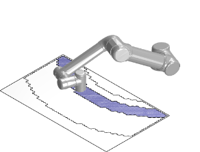
\includegraphics[width = 0.23\columnwidth]{figures/tmech_figures/slwf}
	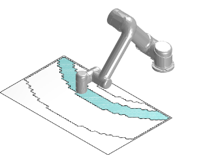
\includegraphics[width = 0.23\columnwidth]{figures/tmech_figures/srwu}
	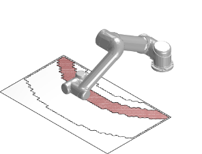
\includegraphics[width = 0.23\columnwidth]{figures/tmech_figures/srwf}
	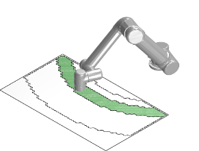
\includegraphics[width = 0.23\columnwidth]{figures/tmech_figures/slwu}
	\label{fig:toy_coverage_example}
}
\subfigure[Valid robot configurations form disjoint sets in joint-space, while their task-space FK mapping images (end-effector poses) may overlap. 
In the example, which for simplicity is illustrated with cells that are maximally $2$-overlapped, 
the resulting task-space graph conveys $N = 11$ undetermined edges constructed as shown by the dashed lines, thus separating the graph into $M = 11$ cells.
To facilitate the understanding whilst limiting clutter in the graph, 3 cells and 2 edges ($i$ and $j$ in dashed blue-green and blue-red respectively) are singled out. 
Solving the NCPP problem for the set of edges in the example can easily reveal all the optimal solutions in this case (two, depicted), demarcating the minimal bound for lift-offs as four. 
It is easy to appreciate how as more colours ``intersect", the algorithmic complexity to find the optimal solutions will soon escalate. % (more intricate examples are provided in Section~\ref{section_experiment}). 
It is also intuitive that should the green colour remain a complete set, both the red and blue colour cells would be split into further disconnected parts, 
leading to extra lift-offs. 
This hints at the fact how to optimally resolve the ``intersecting" of colours can be exploited to reduce the complexity of the solution.
]{
	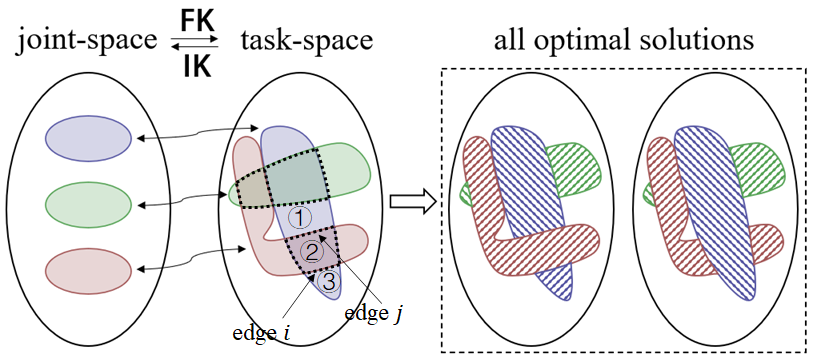
\includegraphics[width = 0.97\columnwidth]{figures/mapping_2}
	\label{fig:toy_coverage_graph_example}
}
\caption{A toy illustration of the problem arising when planning optimal non-revisiting coverage paths with a manipulator: (a) non-revisiting coverage of an object is dictated by the 
available configurations the manipulator can adopt. This leads to (b) disjoint sets in task-space, which conform the input to the NCPP problem. The optimal slicing of these sets leads to minimal discontinuities in tracing the surface with the end-effector. (Please note the above separate examples are independently chosen to best illustrate the problem and do not correspond to each other).
}
\label{fig:mapping}
\end{figure}

\section{Introduction}
\label{section_introduction}
The work in this manuscript is motivated by the \textit{non-revisiting coverage path planning} (NCPP) along the surface of an object~\cite{Paul2013Novel}~\cite{Bhatt2022Automated} with a non-redundant manipulator, as illustrated by~Fig.~\ref{fig:toy_coverage_example}. 
\begin{color}{blue}
% <ty> reviewer comment R2.V thought we used non-repetitive coverage to avoid manipulator lift-offs. This is not correct. Non-repetitive coverage is the task constraint so any resulting must obey this.  
%The NCPP task has realistic importance in that the null of task-space repetitiveness must be guaranteed to avoid undesirable side effects of
NCPP can be paramount in practice to avoid the undesirable effects of  over-coverage, such as excessive removal of surface material form repetitive inspection~\cite{Han2018Tool}~\cite{Wen2022Uniform}, or the formation of fatigue cracks incurred by invasive handling operations such as water jetting~\cite{hassan2018a}.
However, %the path planning for NCPP problem 
coming up with such paths for a manipulator end-effector to track is non-trivial: a continuous task-space coverage path may not admit a continuous, non-singular, collision-free inverse kinematic solution. Likewise, the opposite is also true: a continuous joint-space path may have overlapped task-space images under the nonlinear manipulator kinematics. 
\end{color}

An illustration of these challenges is depicted by the mapping example provided in~Fig.~\ref{fig:toy_coverage_graph_example}, left. 
Given the object's surface, the manipulator, 
the surrounding obstacles in the workcell and their related poses, for each reachable point on the surface there exist a finite number of inverse kinematic solutions in the manipulator configuration space.
Disregarding singular configurations~\cite{Yoshikawa1990Translational}, the collection of all valid configurations form disjoint sets in joint-space. 
When the manipulator transits from one set to another, it adopts a new pose altogether whereby the end-effector (EE) cannot remain on the object, being forcibly detached from the surface. 
%\begin{color}{blue}
This is an undesirable effect for tasks where smoothness and continuity are critical, such as painting~\cite{li2011painting}, deburring~\cite{xie2016grinding}, welding~\cite{lee2011optimal}, scanning~\cite{Giataganas2013Cooperative}~\cite{Huo2021Robotic},  etc.
%, since it is not only suboptimal for the speedy completion of the coverage task, but also introduces unnecessary complicated switches between position and force/torque control~\cite{solanes2018adaptive}. 
%\end{color}
In these instances, the desired solution translates to designing manipulator trajectories such that the end-effector (EE) visits each point on the surface exactly one time, whilst ensuring a minimum number of transitions between joint-space sets, or lift-offs. 

\begin{figure}[t]
\centering
\subfigure[a cell-graph to be solved]{
	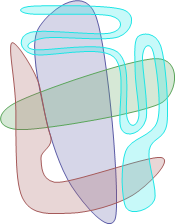
\includegraphics[width = 0.18\textwidth]{figures/cell_graph}
}
\subfigure[the node-graph]{
	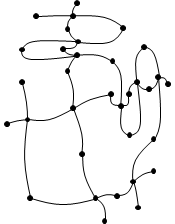
\includegraphics[width = 0.18\textwidth]{figures/node_graph}
}
\caption{Quantitive relationship between the cell-graph notation adopted in the manipulator coverage task and the traditional node-graph concepts in classic graph theory. In this example there are $33$ vertices, $39$ edges, and $8$ faces ($7$ cycles $+$ $1$ outer region reaching the infinity) in the node-graph, which correspond to $33$ cells and $39$ edges in the cell-graph. }
\label{fig:node_graph}
\end{figure}

\begin{color}{blue}
\subsection{Contributions}
\end{color}
Careful examination of the NCPP problem~\cite{Yang2020Cellular} has given birth to a topological graph representation where choosing the optimal manipulator IK solutions for the NCPP task has been transformed into choosing the optimal colours for graph painting. 
Further modelling of the overlap of colours leads in this work to the introduction of a higher-level abstraction, the topological intersection which is the origin of the multiplicity of the optimal solutions. 
See Fig.~\ref{fig:toy_coverage_graph_example} for an intuitive analysis of the phenomenon.  
It is hereby proven that separating the graph into intersection-free sub-graphs leads to all intersections being implicitly enumerated when the sub-graphs are recombined later to calculate the final solutions. 
\begin{color}{blue}
% <ty> reviewer comments R2.VII
The contributions of this paper can be summarised as follows:
\begin{enumerate}
\item We propose a novel solver for the NCCP problem, hereby referred to as the Improved Maximal Continuity Graph Solver (IMCGS). 
The algorithmic complexity is proven to be reduced by a factor of $2^N$ with respect to the state-of-the-art approach in~\cite{Yang2020Cellular}, where $N$ is the number of internal edges in the initial topological graph. 
\item Complexity is substantially enhanced with no trade-offs in the optimality of the solution: the improved graph solver remains globally optimal and complete, thus collecting all optimal solutions as in~\cite{Yang2020Cellular}). 
\item Whilst the improved graph solver is laid out assuming that all cells in the graph are simply-connected, it has already been proven~\cite{Yang2020Nonrevisiting} that for graphs with multiply-connected cells, iterative enumeration can reduce the problem to that of a simply-connected cell graph. Hence the proposed algorithmic improvement is generic to any type of topological graphs.
\item An open source implementation has been supplied, where a supplementary video is also included~\footnote{\textcolor{blue}{https://github.com/ZJUTongYang/imcgs}}. 
\end{enumerate}
\end{color}

\begin{color}{blue}
\subsection{Significance of Contribution}
\end{color}

The significance of the algorithmic improvement can also be revealed by invoking the cell-graph notation promoted in this work and the traditional concept of node-graph in classic graph theory. This equivalence is pictorially shown in Fig.~\ref{fig:node_graph}, whereby a one-to-one correspondence between the cells and edges in a cell-graph and the vertices and edges in a node-graph can be established. The Euler's formula~\cite{Bondy1976Graph} for planar graphs yields: 
\begin{equation}
V - E + F = 2
\end{equation}
where $V$, $E$, and $F$ are the number of vertices, edges, and faces in the node-graph, respectively. 
This relationship highlights the large number of edges in a cell-graph, $F-2$ greater than the number of cells: 
\begin{equation}
N - M = E - V = F - 2
\end{equation} 
It can be observed how in complicated graphs where $F$ will be necessarily large, reducing algorithmic complexity by $2^N$ represents a notable breakthrough. 
This relationship to classic graph theory also points towards a potential contribution in other related research areas besides the manipulator NCPP problem, which is beyond the scope of this work. 


The remainder of this paper is organised as follows. 
Section~\ref{section_related_works} reviews existing literature. 
Section~\ref{section_problem_statement} formally states the non-repetitive manipulator coverage problem, with a revisiting of state-of-the-art graph solver in Section~\ref{section_existing_algorithm}. 
Section~\ref{section_intersection} introduces the concept of \textit{intersection-free} property.
Section~\ref{section_graph_separation} describes concrete steps to separate a graph into intersection-free sub-graphs. 
Solutions to these can then be combined to construct the optimal solutions for the full graph. 
Details about the complexity advantage in solving the problem following the proposed strategy are mathematically proven in Section~\ref{section_complexity}, whilst experimental results from simulations are collected in Section~\ref{section_experiment}. Final concluding remarks are gathered in Section~\ref{section_conclusion}.

\section{Related Works}\label{section_related_works}


Early reports on the generic \textit{coverage path planning} (CPP) problem focused on geometric path designing~\cite{Kaljaca2020Coverage}~\cite{Oriolo2005Motion}, particularly for mobile platforms operating in planar surfaces or near-flat terrains~\cite{Eiben2020Problem}~\cite{Wu2019Energy}, such as boustrophedon~\cite{choset1998coverage} or spiral paths~\cite{hassan2018a}. 
Additional strategies were later proposed that transformed the coverable region into smaller partitions, or \textit{cells}, where continuous coverage paths could be guaranteed. A body of novel partitioning \textit{cellular decomposition} strategies emerged~\cite{Acar2002Morse}~\cite{Acar2006Sensor}~\cite{huang2001optimal}~\cite{Atkar2009Hierarchical}~\cite{Hassan2017Simultaneous}, applied directly to the area to be covered. This is an ineffective strategy when transferred from task to joint-space for manipulator planning since the kinematic mapping between the two spaces is non-bijective: as illustrated in Fig.~\ref{fig:mapping}, the forward kinematic relationship from the configuration space to the surface is surjective (many-to-one) and locally flat (one-to-one from each connected component of the valid configuration space to the surface). 
The problem is further compounded when the EE can only visit each point on task-space once, leading to numerous pose reconfigurations during the motion of the EE~\cite{rososhansky2011coverage}.
Many criteria in the classic CPP problems have been adapted to the manipulator NCPP task, such as time to completion~\cite{lu2020time} or energy consumption~\cite{Mei2006Deployment}, and optimal mobile manipulator pose for a given coverage in task-space has also been investigated~\cite{paus2017a}~\cite{Fan2021Base}~\cite{Kalawoun2018Optimal}.
\begin{color}{blue}
% <ty> reviewer comments 3.II
However, minimising EE lift-offs to decrease the numbers of reconfigurations adopted during a desired task motion has rarely been exploited. 
Specifically for coverage with multi-axis mechanisms, almost all existing works~\cite{Liu2020Optimal}~\cite{Zhou2016Sweep}~\cite{Bhatt2020Incorporating} have neglected the problem and assumed that the target surface is relatively small so as to be entirely embedded into the reachable workcell of a manipulator, which does not generalise well, e.g. for large workpieces. 
\end{color}
Recent propositions in the literature to tackle the problem decomposed the task-space area into a topological graph ensuring continuous joint-space coverage within each cell, and looked for solutions where maximal continuity between cells existed~\cite{Yang2020Cellular}, as intuitively depicted in Fig.~\ref{fig:mapping}. 
\textcolor{blue}{
% <ty>just cueing section IV, as an end of this section
For these cases, all maximally-continuous cellular decompositions were proven to be collectable in a finite number of steps - a relevant observation for this work that will be recalled later in Section~\ref{section_existing_algorithm}. }


\section{Problem Statement}\label{section_problem_statement}
\begin{color}{blue}
% <ty> as a preface
The NCPP task is a generalisation of the classic coverage path planning (CPP) problem, in that for each point in the region to be covered there may be not one but a finite number of valid inverse kinematic solutions to perform the coverage. 
\end{color}
\begin{definition}
(Valid Configuration) A valid configuration is the non-singular~\cite{Yoshikawa1990Translational} collision-free manipulator configuration such that the end-effector rests on the object surface with its orientation parallel to the surface normal. 
\end{definition}
Given the kinematics of a non-redundant manipulator $K$, the pose and surface mesh of the object to be traversed $M$, the obstacles within the robot workspace in the surrounding environment $\{O_i\}$, each point $m\in M$ on the surface can be reached by the EE through a finite number of Inverse Kinematic (IK) solutions $\mathscr{C}(m) = \{c_{m1}, \cdots, c_{mn}\}$. 
\textit{Solving} the graph formally refers to the process of preserving only one of the IK solutions $c_m\in \mathscr{C}(m)$ for each point. 
\begin{color}{blue}
% <ty> It is TMECH20 that modelled NCPP into graph painting problem. So we cannot say the optimal solution is an assignment for each cell a colour before Section IV. 
% <ty> Here we avoid using "merging" cell (as in the initial submission). so we have to reword it
Traversing between discontinuous configurations calls for an EE lift-off for manipulator pose reconfiguration. 
An optimal solution to the NCPP problem in one that admits the minimum number of EE lift-offs during the coverage motion. 
\end{color}

\section{Existing Algorithm}\label{section_existing_algorithm}
\subsection{Definitions}
Given the NCPP problem to be solved, the tuple $(K, \{O_i\}, M)$, the following topological elements are well-defined: 
\begin{definition}
(Colour) Each valid manipulator configuration is represented by a colour, with continuous configurations being assigned the same colour. 
\end{definition}
When singular configurations are disregarded, the forward kinematics mapping from manipulator configuration to end-effector pose space is locally one-to-one. 
Thus, assuming that there is a one-to-one correspondence between an end-effector pose and a point on the surface, the colour of a point on the surface represents the corresponding IK solutions with said colour. 
Early work~\cite{Yang2020Cellular} grouped the points with the same set of possible colours into sub-regions to simplify the problem, namely, cells. 

\begin{definition}
(Cell) A cell $C_1$ (where $1$ represents its index) is a maximally-connected region on the surface, whereby all points within have the same set of possible colours, i.e., 
\begin{color}{blue}
% <ty> for formalism, reviewer comments R3.IV(c)
\begin{equation}
\begin{aligned}
&\forall m, m'\in C_1, m \mbox{ and } m' \mbox{ are task-space continuous} \\
\Leftrightarrow &
\left\{\begin{aligned}
&\mathscr{C}(m) \triangleq \{c_{m1}, \cdots, c_{mn}\}\\
&\mathscr{C}(m') \triangleq \{c_{m'1}, \cdots, c_{m'n'}\}\\
& n = n'\\
& \forall c_{mi}\in \mathscr{C}(m),\ \exists c_{m'j}\in \mathscr{C}(m')\\
&\qquad s.t.\ c_{mi} \mbox{ and } c_{m'j}\mbox{ are joint-space continuous }
\end{aligned}
\right.
\end{aligned}
\end{equation}
\end{color}
The possible colours of a cell is the possible colours of points in the cell. 
\end{definition}
The geometric coverage path within a single cell (e.g., boustrophedon~\cite{choset1998coverage}, spiral path~\cite{hassan2018a}) can be arbitrarily designed with a continuity guarantee, such that when starting from any configuration of choice within the cell, the manipulator will be able to track the chosen coverage path without the need to resort to any end-effector lift-off. 
An edge is delineated by the common boundary between two cells, formally defined as 
\begin{color}{blue}
% <ty> for formalism, reviewer comments R3.IV(c)
\begin{definition}
(Edge) An edge $E_1$ (where $1$ represents its index) is the maximal continuous task-space curve amidst two cells, i.e., within an arbitrary small neighbourhood of the point on edge we may find points belonging to different cells, 
\begin{equation}
\begin{aligned}
E_1 &= E_1(C_i, C_j) \\
&= \{p\in M|\forall (p\in) U_p, \exists m_1, m_2\in U_p, m_1\in C_i, m_2\in C_j\}
\end{aligned}
\end{equation}
\end{definition}
\end{color}

\begin{figure}[t]
\centering
\subfigure[]{
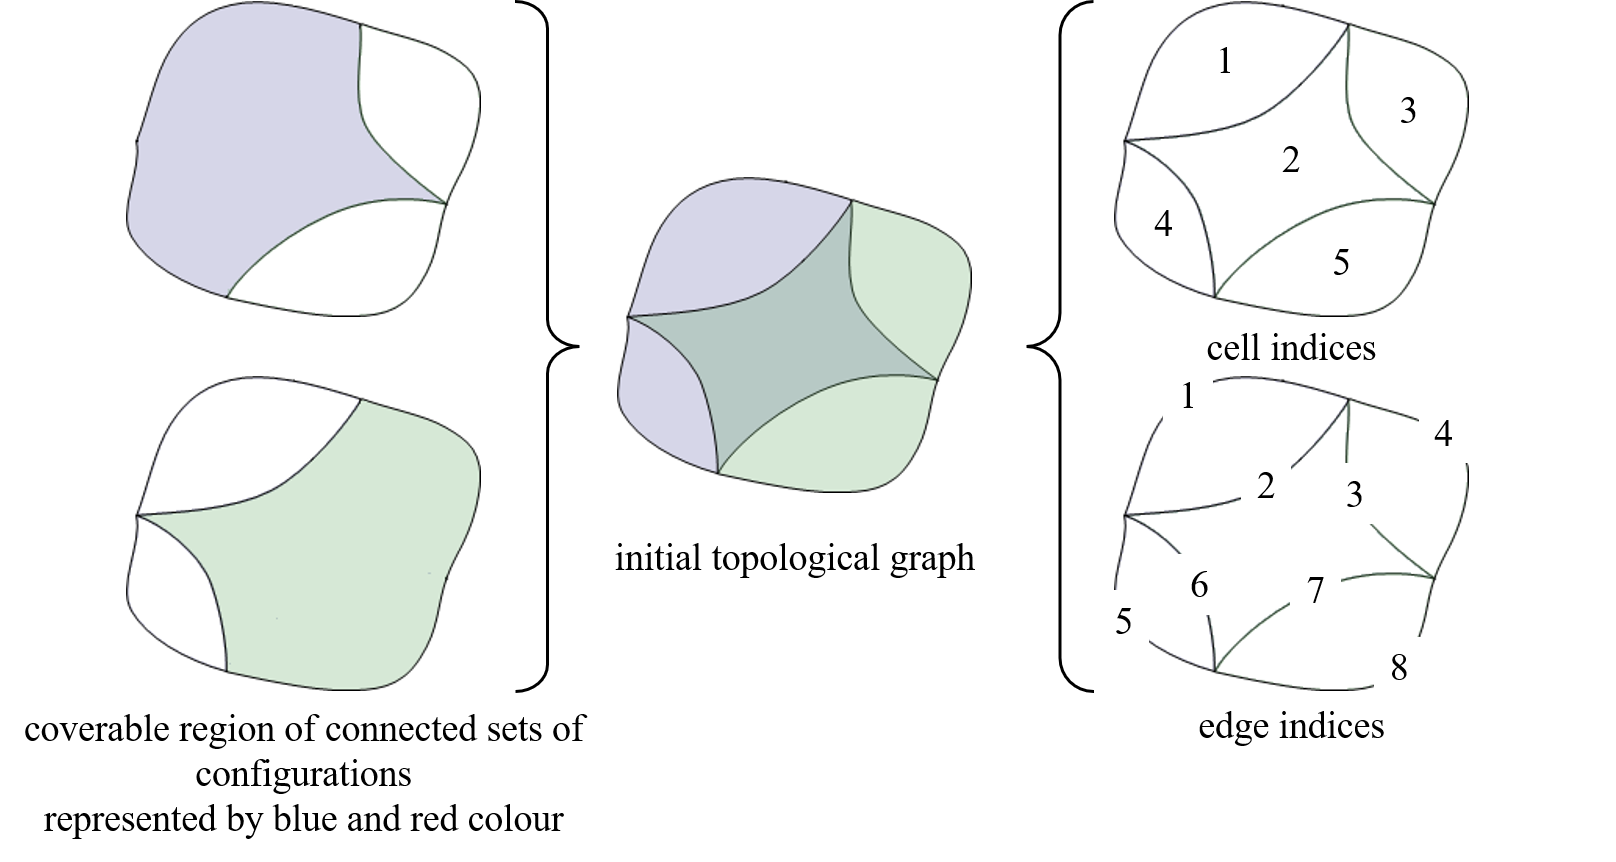
\includegraphics[width=0.48\textwidth]{figures/tmech_figures/simple_case}\label{fig:concepts:a}
}
\subfigure[]{
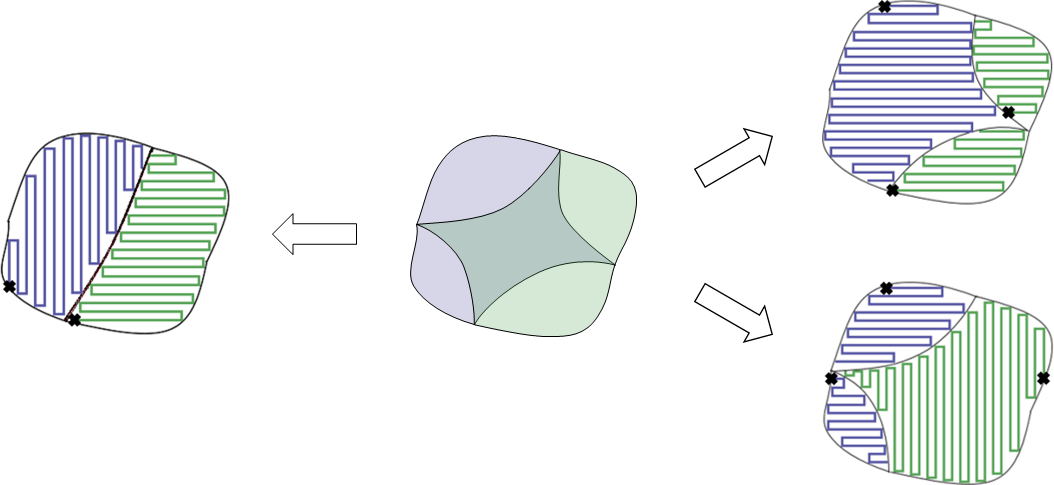
\includegraphics[width=0.48\textwidth]{figures/tmech_figures/simple_solution}\label{fig:concepts:b}
}
\caption{\textcolor{blue}{(a) A simple example to illustrate various cell concepts, where the central cell is the only cell with non-unique possible colours.
(b) Just filling in the central cell with either blue or green colour would be non-optimal (right-hand side examples). 
The resulting solutions will have $3$ connected regions, i.e., $2$ extra EE lift-offs. 
In contrast, dividing the cell into two parts (left-hand side) enables it to connect two pairs of its adjacent cells, leading to an optimal cellular decomposition with $2$ regions (thus only $1$ extra EE lift-off). 
Examples of coverage paths have been illustrated inside each of the final cells, with bold $\bm \times$ denoting the places where the EE would leave the object surface.}
}\label{fig:concepts}
\end{figure}

Finally, the initial topological graph can be constructed by collecting all cells and edges. 
\begin{definition}
(Graph) A graph is the combination of all cells and their connectivity, i.e., the edges. 
\end{definition}

Earlier work~\cite{Yang2020Cellular} has proven that the number of cells in the initial topological graph is finite. 
\begin{color}{blue}
% <ty> reviewer comments R2.VIII, "what exactly is happening in figure 2", and what is "tree pruning" (to be used in the experiment section to explain the difference between theoretical bound and iterations). 

A visual illustration of a cell and its subdivision is supplied in the example shown in Fig.~\ref{fig:concepts}. 
The cell representation in this case can be characterised as 

\begin{equation}
\begin{array}{lll}
\mbox{Cell: }\{{\rm colours}, {\rm edges}\}     &  \multicolumn{2}{l}{\mbox{Edge: }\{{\rm cells}, {\rm constraint}\}}\\
C_1: \{[b], [1, 2]\}     & E_1: \{[-1, 1], \mbox{`'}\} & E_5: \{[-1, 4], \mbox{`'}\}\\
C_2: \{[b, g], [3, 2, 6, 7]\} & E_2: \{[1, 2], \mbox{`'}\} & E_6: \{[2, 4], \mbox{`'}\}\\
C_3: \{[g], [4, 3]\} & E_3: \{[2, 3], \mbox{`'}\} & E_7: \{[2, 5], \mbox{`'}\}\\
C_4: \{[b], [5, 6]\} & E_4: \{[-1, 3], \mbox{`'}\} & E_8: \{[-1, 5], \mbox{`'}\}\\
C_5: \{[g], [7, 8]\}&&
\end{array}
\end{equation}
where the edges connecting to $-1$ are the boundaries of the graph. 
In the initial topological graph, there were no constraints imposed on the edges, so the set is empty (shown in single quotes). 

\subsection{Cell Sub-division and Enumeration}\label{subsection_cell_subdivision}
% <ty> preface
Unlike the usual setting in classic graph theory where nodes are regarded as inseparable entities, cells in this work can be arbitrarily divided into sub-cells (and then painted with different possible colours) to be able to arrive at a better solution. 
Fig.~\ref{fig:concepts:b} shows one such example. 
We refer to the \textit{cell sub-division} process as the designing of cutting paths within a cell. 
\begin{definition}
% <ty> reviewer comments R3.IV(c)
(Cutting Path) The cutting path of a cell is a path starting and ending at the boundary of a cell, enforcing its sides having different colours. 
Taking sub-cells as distinct cells, the cutting path is equivalent to a manually created edge. 
\end{definition}
\end{color}

Moreover, the following lemma ensures the finiteness of all possible topological-distinct cellular decompositions. % <ty> We cannot copy the original sentence as it is too long


\begin{color}{blue}
% <ty> reviewer comments R1.VI, R2.III, 
\begin{lemma}\label{lem:principles}
The following principles for designing cutting paths in a cell have been proven in~\cite{Yang2020Cellular}: 
\begin{enumerate}
\item We only need to consider cutting paths which connect edge endpoints. 
\item We only need to consider cutting paths which go across edges. 
\item We only need to consider intersecting cutting paths. 
\end{enumerate}
\end{lemma}
\end{color}

\begin{color}{blue}
% <ty> Just connect paragraphs
A finite-step graph solver has been proposed to collect all optimal solutions.
In each iteration, for an unpainted cell (say it has $\alpha$ edges and $K$ possible colours), we firstly enumerate all its possible cell sub-divisions (say there are $E = E(\alpha)$ ways) which construct different branches. 
\end{color}
It has been shown how a binary array of length $\alpha$ can be used to index all possible different cell sub-divisions~\cite{Yang2020Cellular}, whereby $0$ at a given position enforces the cell having a different colour to its adjacent cell, whilst $1$ compels the same choice of colour. 
However, as supported by the illustrative example shown in Fig.~\ref{fig:many_to_one}, for one of the edge solutions ``$1111$" and $2$ possible colours available for painting, the binary array does not uniquely represent a valid painting solution: the cell may be divided into parts with differing colours, while each part themselves connect to their two adjacent cells. 
% \begin{color}{red}
% Note that binary enumerations with $\alpha$ letters listing all possible connectedness of edges are not enough to represent all solutions: 
% As supported by the illustrative example shown in Fig.~\ref{fig:many_to_one}, 
% for one of the edge solutions ``$1111$" and $2$ possible colours available for painting, the cell may be non-divided or divided into parts with differing colours. 
% \end{color}
Hence, in generic, there may be up to $E(\alpha)\cdot 2^\alpha\cdot K^{\max\{\alpha - 2, 1\}}$ different branches after solving an $\alpha$-edge cell with $K$ possible colours. 
In the next iteration, an unsolved branch is selected, and an unsolved cell within it, and repeat the same process. 


\begin{figure}[t]
\centering
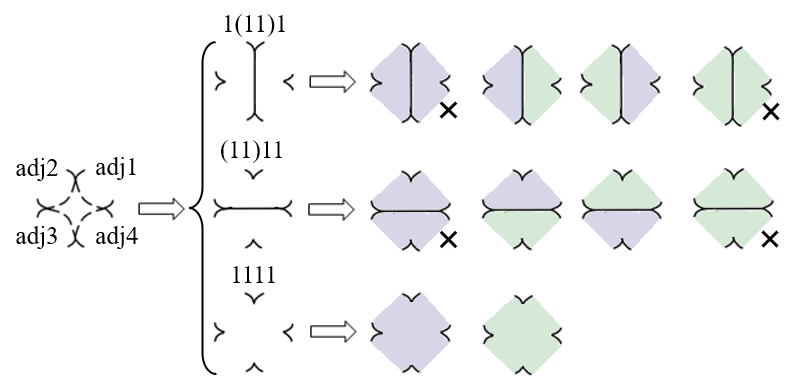
\includegraphics[width = 0.48\textwidth]{figures/many_to_one_4}
\caption{An illustration of the many-to-one relation between edge and painting solutions. 
Let a cell with $4$ adjacent cells (a $4$-edge cell) have 2 possible colours ``blue" and ``green", then $\alpha = 4, K = 2$. From the point of view of solving edges, the binary number $1111$ specifies one solution, but the corresponding valid painting solutions are multiple, $6$ to be precise: there can be no cell subdivisions, or $E=2$ ways to divide the multi-edge cell into $3$-edge sub-cells, and $\alpha-2 = 2$ sub-cells are generated which can be filled with the $K (=2)$ possible colours. After enumerating $E\cdot K^{\max\{\alpha-2, 1\}}$ cases, four of them are removed (adjacent sub-cells are separated by cutting paths thus cannot be painted by the same colour), shown crossed-out, leaving the remaining 
six valid painting solutions.
}
\label{fig:many_to_one}
\end{figure}

\begin{color}{blue}
% <ty> reviewer comments R2.VIII, "what exactly is happening in figure 2", and what is "tree pruning" (to be used in the experiment section to explain the difference between theoretical bound and iterations). 
An example for this operation in the optimal graph solution shown in Fig.~\ref{fig:concepts:b} can be listed as follows:  
\begin{equation}
\begin{array}{lll}
\multicolumn{2}{l}{\mbox{(only changed elements are listed)}} &\\
C_2:\{[b, g], [3, 2, 6, 7]\}     & E_2:\{ [1, 2], \mbox{`'}\} & E_6:\{[2, 4], \mbox{`'}\}\\
\multicolumn{3}{l}{\Downarrow (\mbox{cell subdivision})\Rightarrow \mbox{(other branches)}\cdots}\\
C_2:\{[b, g], [3, 9, 7]\} &E_2:\{[1, 6], \mbox{`'}\}&E_6:\{[4, 6], \mbox{`'}\}\\
C_6:\{[b, g], [2, 6, 9]\} &E_9:\{[2, 6], \mbox{`0'}\}&  \\
\multicolumn{3}{l}{\Downarrow (\mbox{tree pruning, the adjacent cells must be connected})}\\
C_2:\{[b, g], [3, 9, 7]\} &E_2:\{[1, 6], \mbox{`1'}\}&E_6:\{[4, 6], \mbox{`1'}\}\\
C_6:\{[b, g], [2, 6, 9]\} &E_9:\{[2, 6], \mbox{`0'}\}&  \\
\multicolumn{3}{l}{\Downarrow (\mbox{tree pruning, the colour of sub-cell is constrained})}\\
C_2:\{[b, g], [3, 9, 7]\} &E_2:\{[1, 6], \mbox{`1'}\}&E_6:\{[4, 6], \mbox{`1'}\}\\
C_6:\{[b], [2, 6, 9]\} &E_9:\{[2, 6], \mbox{`0'}\}&  \\
\multicolumn{3}{l}{\Downarrow (\mbox{tree pruning, sub-cells cannot have the same colour})}\\
C_2:\{[g], [3, 9, 7]\} &E_2:\{[1, 6], \mbox{`1'}\}&E_6:\{[4, 6], \mbox{`1'}\}\\
C_6:\{[b], [2, 6, 9]\} &E_9:\{[2, 6], \mbox{`0'}\}&  \\
\multicolumn{3}{l}{\mbox{(all cells have a unique color, }} \\
%\multicolumn{3}{l}{\qquad\qquad\mbox{there are 2 connected regions)}}
\multicolumn{3}{l}{\mbox{there are 2 connected regions)}}
\end{array}
\end{equation}



\end{color}

\subsection{Algorithmic Complexity}

Let there be $M$ topological cells and $N$ internal topological edges in the modelled graph to be solved. The number of edges for the $i$-th cell is $\alpha_i$, and denote the number of possible colours to fill cell $i$ as $K_i$. 
Considering a worst case scenario, let there be $E_i$ different ways to divide cell $i$ into $(\alpha_i-2)$ sub-cells, then $E_i\cdot K_i^{\max\{\alpha_i-2, 1\}}\cdot 2^{\alpha_i}$ steps are required for a single cell. Iteratively enumerating each cell and noting that each edge will only be enumerated once in the process, the upper bound of algorithmic complexity can be calculated as
\begin{equation}\label{equ:tmech_complexity}
\prod\limits_{i=1\atop\alpha_i \geq 4}^{M}E_i\cdot \prod\limits_{i = 1}^M K_i^{\max\{\alpha_i-2, 1\}} \cdot 2^N
\end{equation}


\begin{figure}[t]
\centering
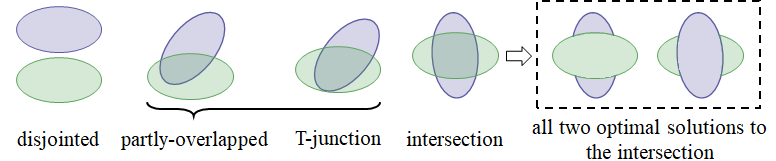
\includegraphics[width = 0.48\textwidth]{figures/basic_shape_3}
\caption{Illustration of the basic relationships between the reachable area for a two-colour case. 
In all but the intersection scenario, each colour can keep itself fully connected. 
T-junction can be seen as a special instance of the generic partly-overlapped case, as it can be transformed back to the generic case through continuously modifying the boundary of the colours. 
Only the intersection case needs solving, and it is apparent that the two optimal solutions are not topological equivalent: they have a different number of connected regions for each colour, depending on whether the blue or the green colour is chosen in the intersecting area.}
\label{fig:basic_shape}
\end{figure}

\begin{figure}[t]
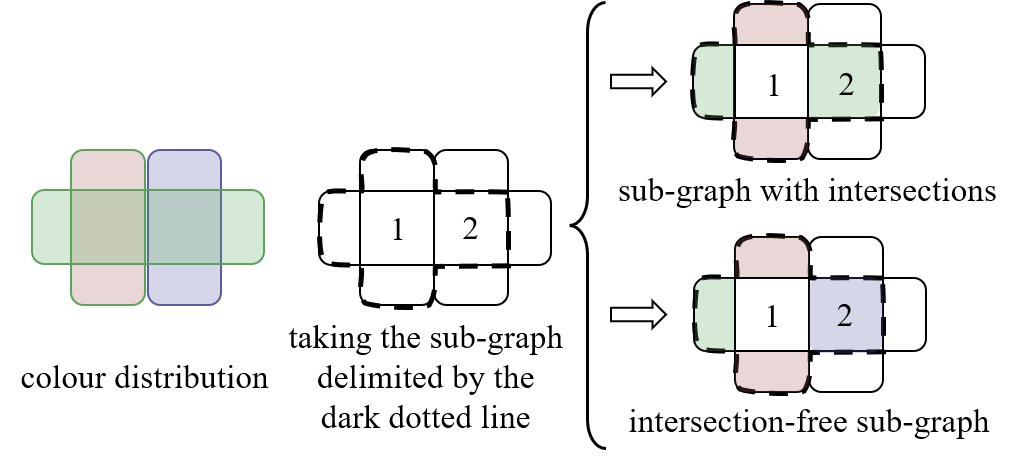
\includegraphics[width=0.48\textwidth]{figures/simple_intersections_indexed}
\caption{Illustration of intersection-free sub-graph. 
By definition, the intersection-free property is subject to the colouring of boundary cells. 
In this example, taking the sub-graph delimited by the dark dotted line, if cell $2$ is assigned as blue, then the sub-graph is intersection-free, as cell $1$ being filling in with red is the only optimal solution. Or else, with cell $2$ being in the green colour, either green or red in cell $1$ will constitute an optimal solution of the sub-graph, where by the sub-graph is not intersection-free. }\label{fig:simple_intersection}
\end{figure}


\section{Proposed Method: Optimality via ``Topological Intersections''}
\label{section_intersection}

\begin{color}{blue}
% <ty> reviewer comments R3.IV(b)
To construct the globally optimal painting schemes of the topological graph, one will naturally consider how the solution of a part in the graph contributes to that of the entire graph. 
\end{color}
Typically, for the simplest case, the coverable area of two colours may be fully disjointed, partly overlapped, or intersected, as shown in Fig.~\ref{fig:basic_shape}. 
There are two obvious optimal solutions to the right-most intersected case: 
filling in the central cell fully with either blue or green. 
It can be observed how colours can be kept connected in the disjointed and partly overlapped cases, but critically in the intersection case one colour being connected will truncate the other colour in two parts.
Intuitively, having all other parts of the graph been already painted, the remaining part of the graph should be painted such that it maximally ``connects" its adjacent cells. 
In this regard, the concept of intersection-free graphs plays a crucial role.  


\subsection{Intersection-free Sub-graphs}
\begin{color}{blue}
% <ty> reviewer comments R3.IV(h)
\begin{definition}
(Sub-Graph) A sub-graph is a connected subset of cells in the graph, together with all edges that connect these cells. 
The adjacent cells of the sub-graph are the cells adjacent to any cell within the sub-graph. 
The boundary of a sub-graph is the set of edges between cells inside/outside the sub-graph, listed in order. 
\end{definition}
To simplify the discussion, all sub-graphs in the paper are assumed simply-connected, hence the adjacent cells of a sub-graph are well-ordered, and the boundary of a sub-graph is a close chain of edges. 
\end{color}

\begin{definition}
(Boundary Cell, Internal Cell) Boundary cells are the cells which have edges forming the boundary of the sub-graph. The remaining cells are internal cells which have no edge exposed to the sub-graph boundary. 
\end{definition}

\begin{color}{blue}
% <ty> reviewer comments R3.IV(a)
%We formally define \textit{intersection-free} as the uniqueness of optimal solution of a sub-graph subject to a specified colour assignment of its boundary cells.
We formally define the \textit{intersection-free} property of a sub-graph by the peculiarity that, subject to a specified colour assignment of its boundary cells, the optimal solution for its internal cells is unique.

\begin{definition}
(Intersection-free Sub-graph) Let a sub-graph have $r$ boundary cells and $s$ internal cells, indexed as $1, \cdots, r, r+1, \cdots, r+s$ and having $K_1, \cdots, K_{r+s}$ possible colours. 
A sub-graph can be distinguished as an intersection-free sub-graph only if 
\begin{enumerate}
\item $K_1 = \cdots = K_r = 1$.
\item There exists only one topology-distinct optimal solution among all enumerations of internal cells $r+1, \cdots, r+s$ for the sub-graph. 
\end{enumerate}
\end{definition}
\end{color}

\begin{figure}[t]
\centering
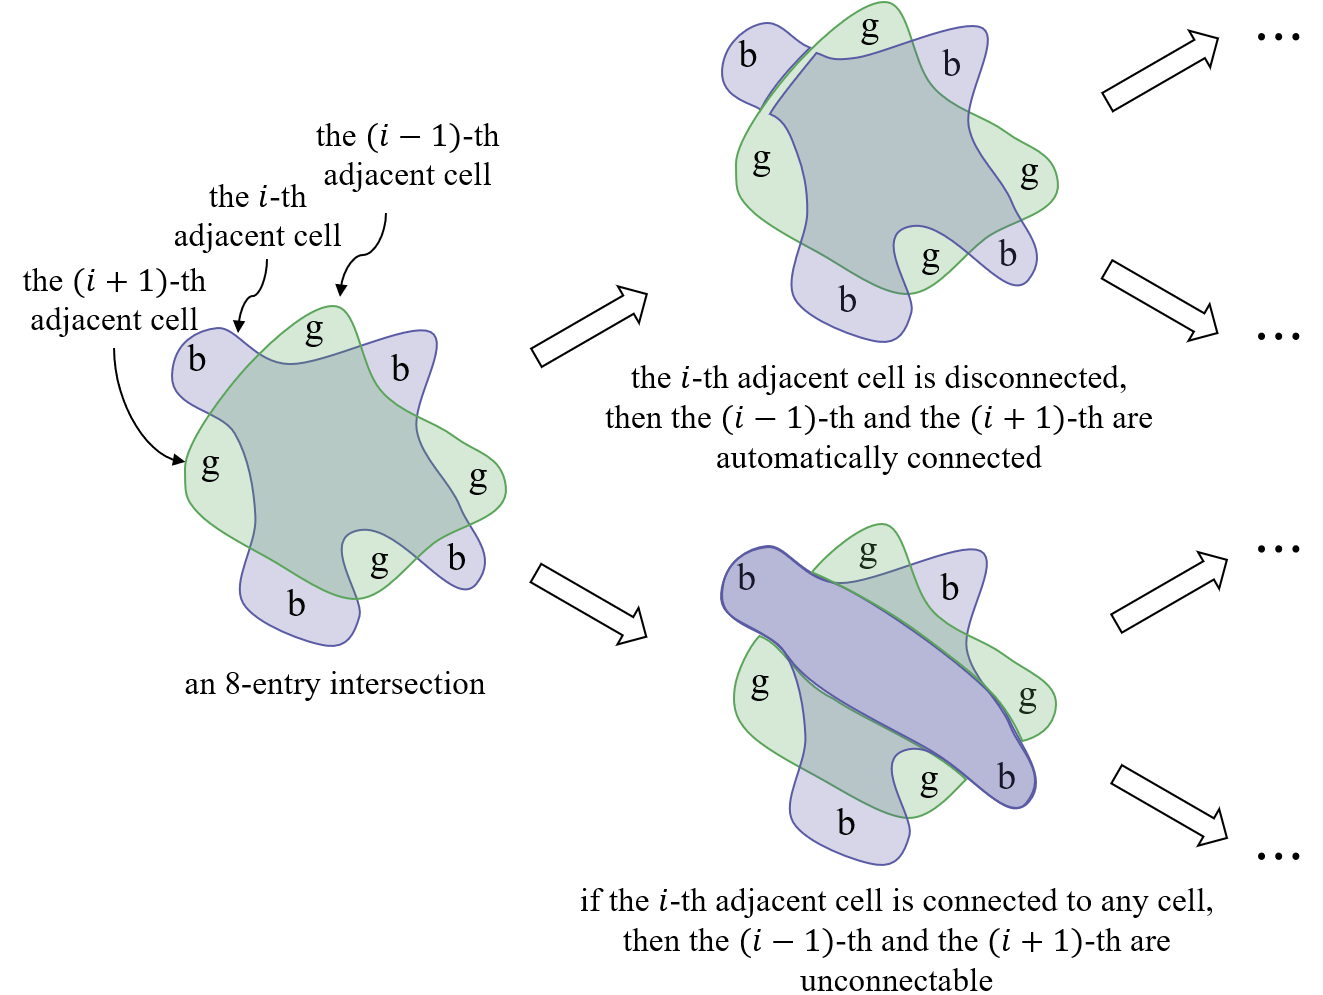
\includegraphics[width = 0.48\textwidth]{figures/new_multi_entry_2}
\caption{
An example of intersection with $8$ adjacent cells is depicted on the left. 
The figure also illustrates the process of solving an intersection with a simpler example where adjacent cells have been assigned alternate colours ``b(lue), g(reen), b, g, $\cdots$". 
It is apparent from the two token scenarios shown that an exhaustive enumeration will be required to obtain all optimal cellular decompositions.
More generically, let the intersection have an even number (say $n$) of adjacent cells, with consecutive adjacent cells having been assigned alternate colours, ``b(lue), g(reen), b, g, $\cdots$". 
It is observed that for each adjacent cell (say the $i$-th, labelled cyclically), if it is connected to any other adjacent cell through the intersection, then another two adjacent cells, $(i-1)$ and $(i+1)$, cannot be connected. 
So the minimal number of connected regions is $\frac{n}{2}+1$. 
However, note that whilst the optimal number can be directly deduced, to get all optimal cellular decompositions the intersection still needs to be enumeratively solved. 
For the $i$-th adjacent cell, two scenarios must then be separately regarded: 
(a) keeping itself disconnected so that adjacent cells $(i-1)$ and $(i+1)$ can be connected (top-right), or (b) connecting it to other adjacent cells (bottom-right). 
Both of them go to optimal cellular decompositions and they are topologically distinct.
}\label{fig:multi_entry}
\end{figure}

\begin{color}{blue}
% <ty> Necessary explanation, or else this subsection only has definitions. 
The concept of intersection-free sub-graphs is illustrated in Fig.~\ref{fig:simple_intersection}. 
The underlying reason for the multiplicity of optimal solutions is the different ways that a sub-graph may connect its adjacent cells, even with equal number of connections. 
As different adjacent cells become connected and disconnected through the sub-graph, the number of connected regions of each colour differs. 
Hence, these optimal solutions are topologically distinct and have to be collected by enumeration. 

In fact, all sub-graphs with intersections have to be enumerated in order to identify all optimal solutions. 
Refer to the illustration in Fig.~\ref{fig:multi_entry} where all enumerations of the internal cell may constitute an optimal solution, 
the illustration in Fig.~\ref{fig:local_combined} where the optimal of sub-graph has no relation to the global optimal solution of the whole graph, 
and the illustration in Fig.~\ref{fig:two_overlapped_graph} where all possible combinations of all enumerations of cells form an optimal solution of the whole graph, by which the necessity of enumeration is indicated. 

\end{color}

\begin{figure}[t]
\centering
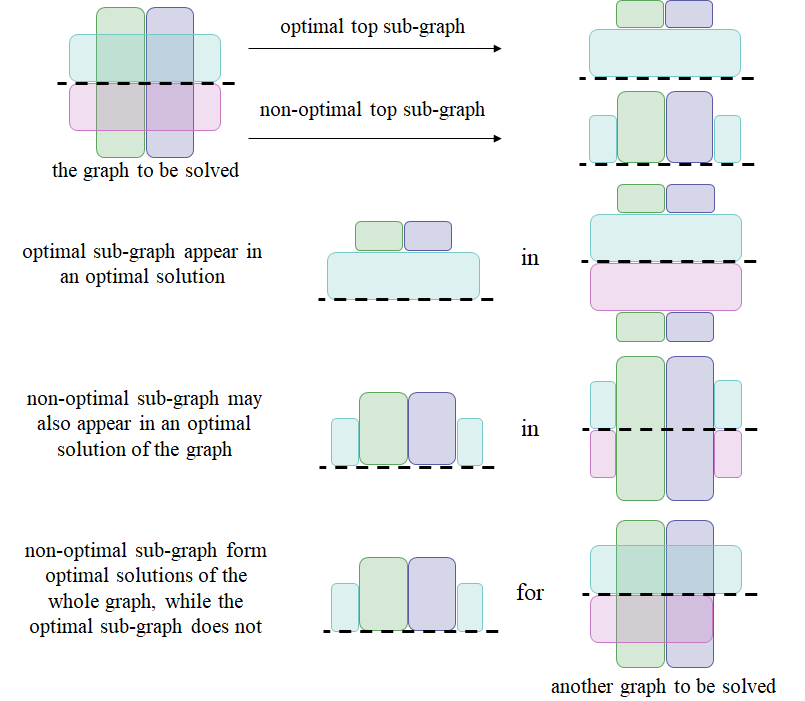
\includegraphics[width=0.48\textwidth]{figures/local_combined}
\caption{Separating the graph through the dashed line, we show the optimal solution and a non-optimal solution of the sub-graph. It is noticeable that both of them form optimal solutions of the original graph. An in the bottom case, as a sub-graph of another graph, the non-optimal sub-graph can form optimal solutions while the optimal sub-graph cannot do so. }\label{fig:local_combined}
\end{figure}

\begin{figure*}[t]
\centering
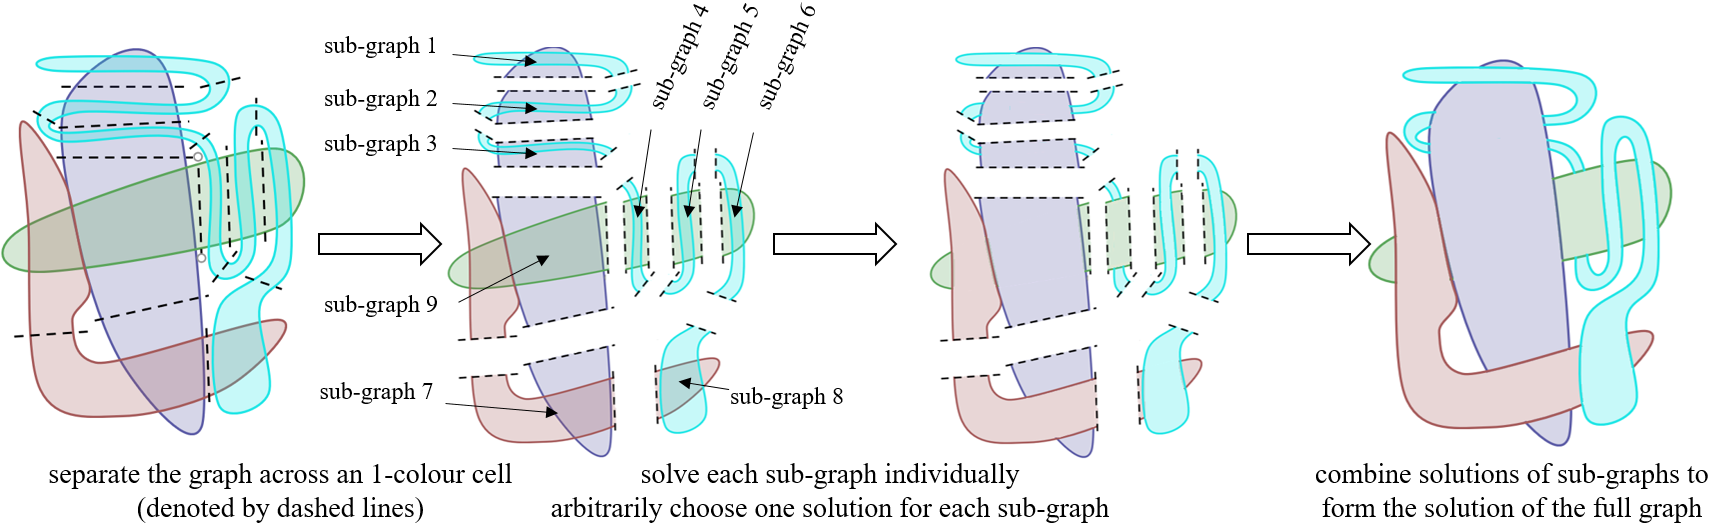
\includegraphics[width=\textwidth]{figures/two_overlapped_graph_2}
\caption{
A maximally 2-overlapped graph to show the role of intersections. 
The key step is to separate the full graph (left) into $9$ sub-graphs through $1$-colour cells, shown with dashed graph separating lines. 
Sub-graph $1$-$8$ has been shown to have two optimal solutions, while sub-graph $9$ gets a unique optimal solution after enumerative solving. 
Whatever solution gets chosen in each sub-graph, when two sub-graphs are combined, the two $1$-colour sub-cells separated by the dashed line re-join together, resulting in a reduction of one on the number of continuous regions. 
In total $4+(3\times 8)=28$ connected regions can be observed after solving the sub-graphs individually, combined with cost $-15$ (number of dashed lines). The nonrepetitive coverage problem of this graph ends up with $28-15=13$ connected regions, i.e., $12$ lift-offs. 
Note that no intersections in the full graph are avoided when solving all the sub-graphs. And different choices of the solution for each sub-graph will double the number of optimal solutions of the full graph: there will be $2^8=256$ optimal solutions to the graph.
In other words, all sub-graphs with intersections have to be enumerated. 
}
\label{fig:two_overlapped_graph}
\end{figure*}

\section{\textcolor{blue}{Proposed Method: Graph Pre-separation}}
\label{section_graph_separation}
% <ty> reviewer comments R3.V
It has been discussed how disregarding the position of intersections and how to solve them leads to exhaustive implicit enumeration when all edges and cells are enumerated. 
On the other hand, exploiting the interesting complex scenarios that analysing the topology between different colours offer will attenuate this problem. 
An efficient mechanism \textcolor{blue}{called IMCGS} to separate a graph into intersection-free sub-graphs is described in this section. 
The reader is referred to the algorithm pseudocode given in \textbf{Algorithm}~\ref{alg:1}.

\subsection{Definition of Strips}\label{sec:strip_solution}



\begin{definition}\label{def:strip}
(Strip) A strip is a sub-graph designed such that
\begin{enumerate}
\item Each internal cell has at most $3$ connectable adjacent cells. 
\item Internal cells are non-adjacent or disconnectable.  
\end{enumerate}
\end{definition}

\begin{proposition}\label{proposition:strips}
\textcolor{blue}{
% <ty> Now the intersection-free property is subject to the assignment of boundary cell colours. So we need to change this proposition
Given any possible colour of the boundary cells of a strip, the strip is an intersection-free sub-graph. }
\end{proposition}
\begin{proof}
It is observed that for a sub-graph with intersections, its internal cell must be able to be assigned colours such that different pairs of painted adjacent cells can be connected. 
In other words, it needs to have at least $4$ connectable adjacent cells. 
Then its opposite becomes a sufficient condition for distinguishing intersection-free sub-graphs: 
If condition 1) in \textbf{Definition}~\ref{def:strip} is satisfied, then there can not possibly be multiple optimal choices of colours. 
In noting that two internal $3$-edge cells may form a $4$-edge cell which breaks this criterion, condition 2) is required. 
\end{proof}

\begin{color}{blue}
% <ty> We only said the solution for internal cells is unique, but didn't say what it is. So we add this. 
Now that the optimal solution for the internal cell of an intersection-free sub-graph is unique, finding it is easy: choosing for each internal cell the colour that maximally connects its adjacent cells. 
See Fig.~\ref{fig:characteristic_string} as an example. 
In this case, if internal cell $1$ can be painted in blue, then it is optimal to be assigned as blue. 
Otherwise, if it can be painted in green, then green. 
Finally, any other colour if there is can also be chosen. 
This solution is simply represented by the priority of choice: blue $>$ green $>$ other colours. 
For internal cell $2$, the solution is: green $=$ red $>$ other colours. 
\end{color}


\begin{figure*}[t]
\centering
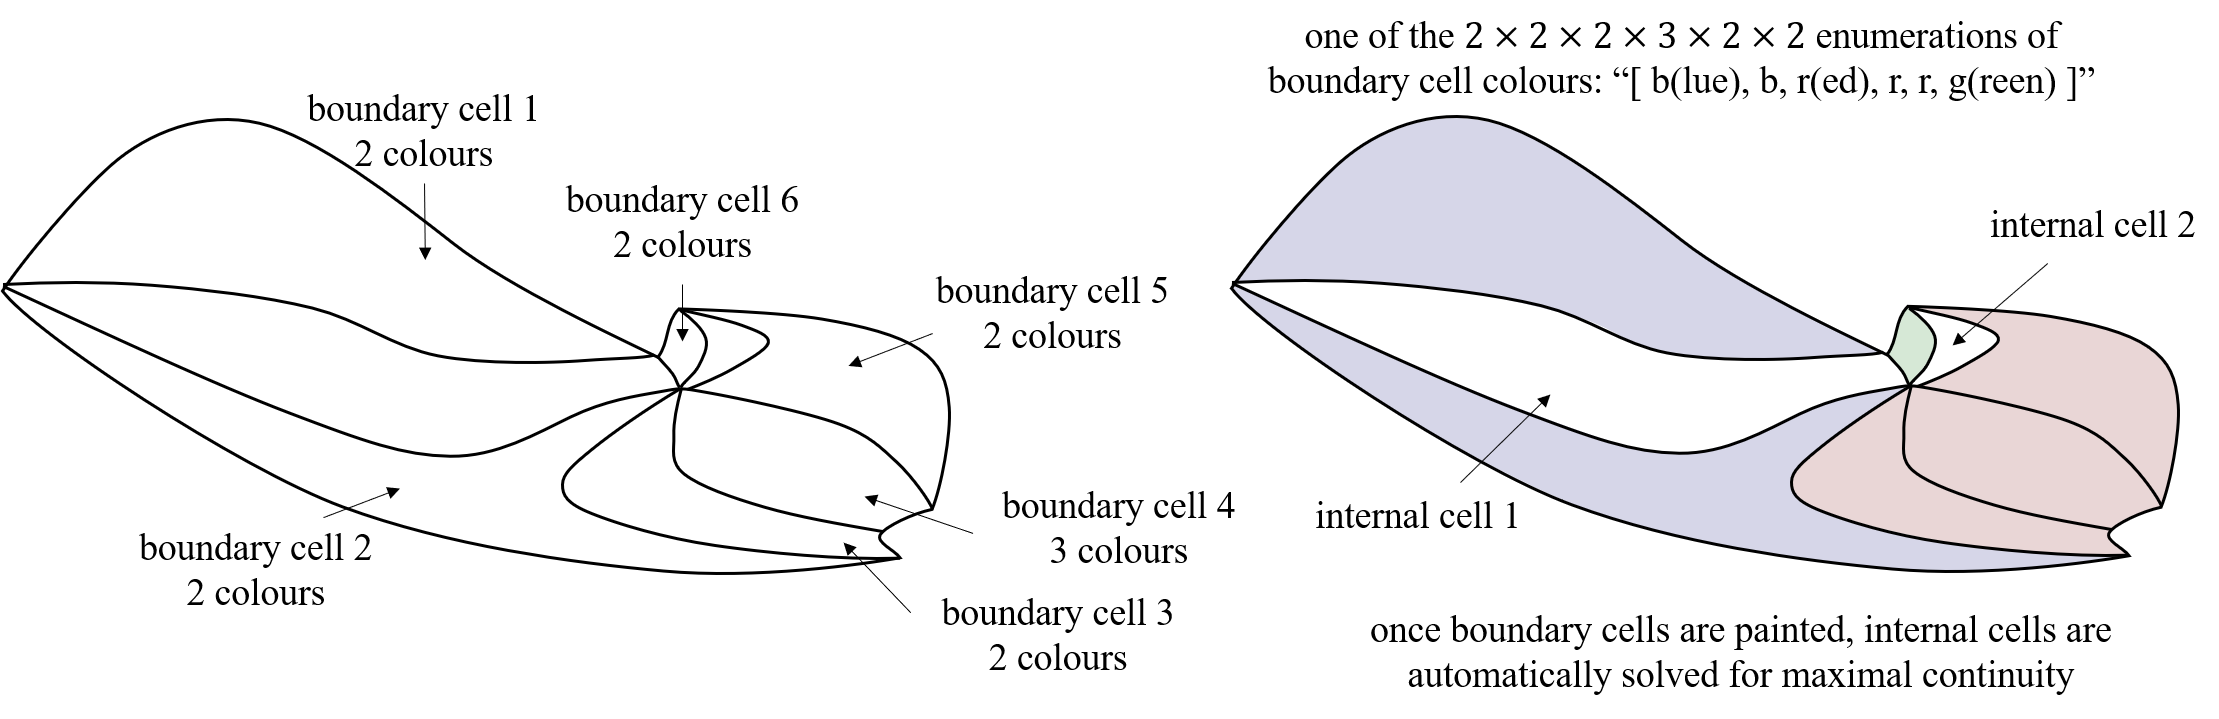
\includegraphics[width=0.9\textwidth]{figures/characteristic_string_3}
\caption{An intersection-free graph. 
The internal cell $1$ will choose blue $>$ green $>$ other colours. 
The internal cell $2$ will choose green $=$ red $>$ other colours.
}\label{fig:characteristic_string}
\end{figure*}

\begin{figure}[t]
\centering
\subfigure[]{
	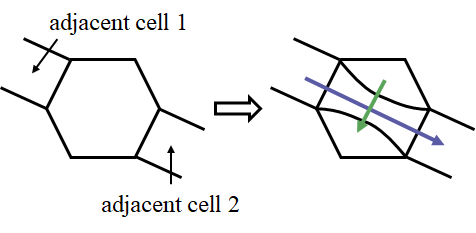
\includegraphics[width=0.22\textwidth]{figures/constraint_violation_a_2}
}
\subfigure[]{
	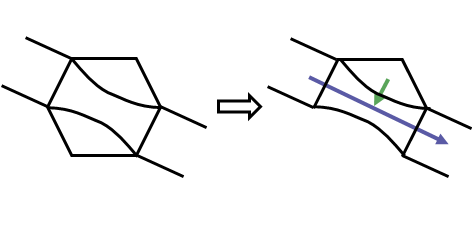
\includegraphics[width=0.22\textwidth]{figures/constraint_violation_b_2}
}
\caption{(a) Illustration of constraint violation due to cell sub-divisions in sub-graphs. One sub-cell will have four adjacent cells. (b) If a cell is scheduled to be divided, it should first be divided and then followed by constructing the intersection-free sub-graphs.}
\label{fig:constraint_violation}
\end{figure}



Since non-adjacency of internal cells in sub-graphs will be enforced, but cell sub-divisions after sub-graphs have already been constructed, this constraint may be violated (see Fig.~\ref{fig:constraint_violation} for an illustration of this scenario).
So let at this point all cells be assumed properly divided before applying the algorithm. As such, 
all cells contained in the sub-graphs can only be seen as a whole, and be filled with the same colour. 


\begin{algorithm}[t]
    \caption{IMCGS}\label{alg:1}
    \begin{algorithmic}[1]
        \Require The initial graph $G = (\{C_i\}_{i = 1}^M, \{E_j\}_{j = 1}^N)$  
        \Ensure All solved graphs $\{result\}$  
\For{all divisions of cell $1$} 
\If{non-optimality is detected}
\State \textbf{continue}
\EndIf
\State $\ddots$
	\For{all divisions of cell $M$}
	\If{non-optimality is detected}
	\State \textbf{continue}
	\EndIf
	\State // Graph Separation into Strips (Section~\ref{section_graph_separation})
		\While{the graph is not intersection-free}\label{alg:separation_start}
		\State Choose a cell to be in the new strip
		\State Attach new cells satisfying constraints
		\State separate the strip from the graph
		\EndWhile\label{alg:separation_end}
		\State // Let there be $n$ strips generated
		\For{all enumerations of boundary cells}
		\State Assign optimal colour choice to internal cells\label{alg:combining_start}
		\If{it is better than $\{result\}$}
		\State $\{result\} = \varnothing$
		\State push $S$ into $\{result\}$
		\Else
		\If{it is currently optimal}
			\State push $S$ into $\{result\}$
		\EndIf
		\EndIf\label{alg:combining_end}
		\EndFor
	\EndFor
\State $\udots$
\EndFor% cell 1 sub-division
    \end{algorithmic}  
\end{algorithm}


\begin{figure*}[t]
\centering
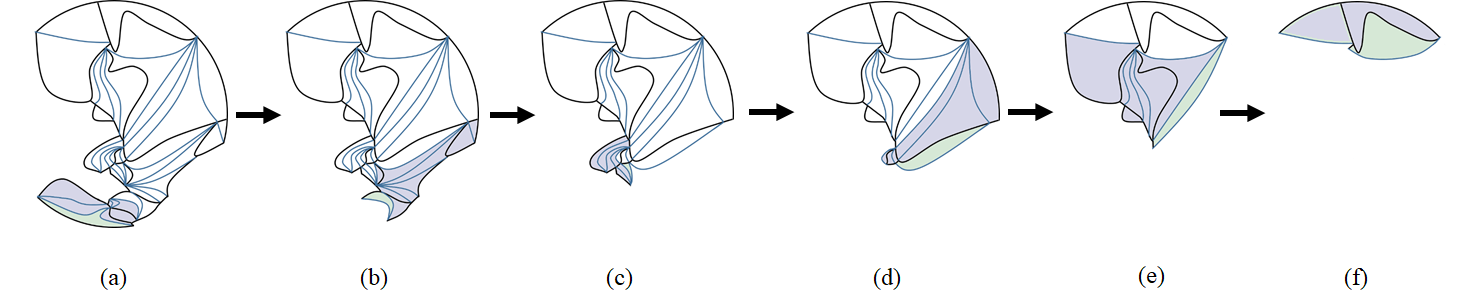
\includegraphics[width=0.96\textwidth]{figures/steps_2}
\caption{\textcolor{blue}{
% <ty> reviewer comments R1.VII(b)
Step-by-step illustration of the separation of a topological graph into intersection-free strips.}
The light green cell is the first one selected to form a new strip, and all light purple cells are then inserted into the same strip. The graph ends up with $6$ separated strips. See also Fig.~\ref{fig:complicated_graph}.}
\label{fig:steps}
\end{figure*}

\begin{figure*}[t]
\centering
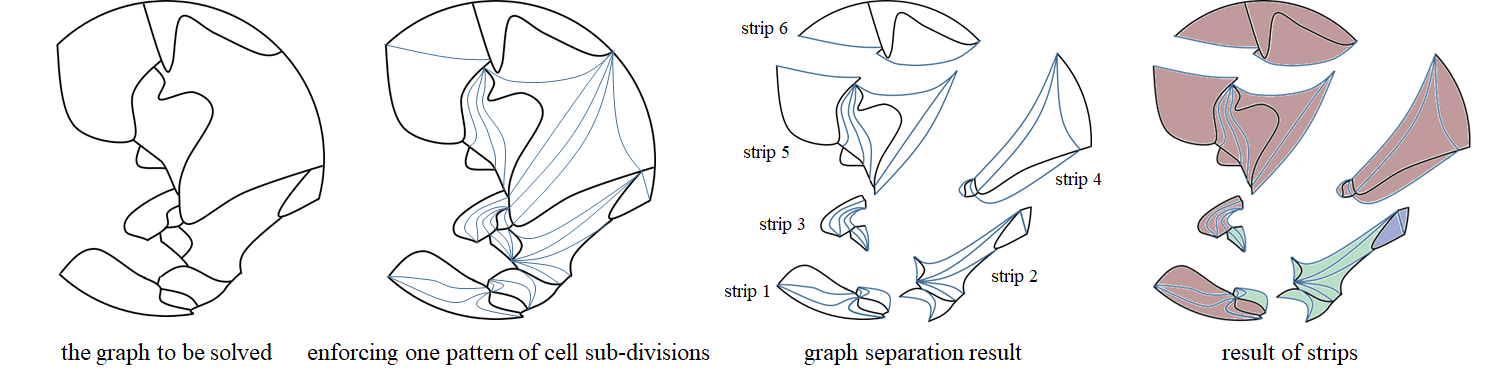
\includegraphics[width =0.96\textwidth]{figures/graph_separation_3}
\caption{Illustration of how an unsolved graph is separated into strips. }\label{fig:complicated_graph}
\end{figure*}



%With all internal cells being isolated, a graph satisfying the above two constraints is referred to as a \textit{strip}. 


\subsection{Graph Separation into Strips}
At this point in the start of the separation process it can be safely assumed that all multi-edge cells have been divided. 
One boundary cell is first selected and regarded as an element of strip $1$, shown in light green in Fig.~\ref{fig:steps}(a).
Each cell adjacent to the strip is checked to validate whether accommodating the cell into the strip will violate the strip constraints (\textbf{Definition}~\ref{def:strip}). Otherwise it is inserted. 
When no further cells can be inserted, the construction of strip $1$ is deemed finished. 
In this example, as shown in Fig.~\ref{fig:steps}(a), adjacent cells are iteratively inserted to strip $1$ which are shown in blue. If one more cell is inserted, then the boundary cell $5$ (illustrated in detail in Fig.~\ref{fig:characteristic_string}) will become an internal cell which is adjacent to the internal cell $2$, so the construction of strip $1$ terminates.  

To construct strip $2$ (Fig.~\ref{fig:steps}(b)), a cell (shown in light green) adjacent to strip $1$ is selected, then its adjacent cells are checked one-by-one to see whether they can be inserted respecting the conditions in \textbf{Definition}~\ref{def:strip}. 
After that, another cell in the left-out graph is chosen into strip $3$ (Fig.~\ref{fig:steps}(c)), and other cells are again checked and attempted to be inserted into strip $3$, and so on. 
By iteratively considering adding the adjacent cells to the previous strip into the current strip and adding more cells satisfying the two constraints, 
the whole graph can be finally separated into strips, as shown in Fig.~\ref{fig:complicated_graph} where the graph is separated into $6$ strips. (The process corresponds to line \ref{alg:separation_start} $\sim$ line \ref{alg:separation_end} in \textbf{Algorithm} \ref{alg:1}.) 
Note that there is no extra memory cost for this step - we are to enumerate all boundary cells of all strips and leave all internal cells un-enumerated, hence we need not physically manipulate the graph into strips as shown in figures, but simply mark all internal cells and skip them whilst enumeration. 
Besides, the enumeration can still be accessed in the depth-first manner. 
\begin{color}{blue}
An implementation in C++ has been open sourced at: 

\url{https://github.com/ZJUTongYang/imcgs}
\end{color}

\subsection{Full Graph Solution}
All the solutions for each strip are enumerated via iterating through all possible combinations of colours of its boundary cells, and for each enumerated case, the optimal colour of each internal cell is assigned. 
Picking up one solution from each sub-graph, they are combined to form a solution of the original graph. 
The edges identified during the graph separation process are automatically solved by comparing the colour of its two adjacent cells. 
A cost is calculated whose physical meaning is the number of connected regions in the painted part of the (combined) sub-graphs~\cite{Yang2020Cellular}. 
Once the original graph is re-constructed, the number of connected regions in the solution is fully known. 
Its optimality can be trivially judged against all possible combinations of sub-graph solutions to reach a set with all the optimal solutions. (line \ref{alg:combining_start} $\sim$ line \ref{alg:combining_end} in \textbf{Algorithm} \ref{alg:1})


% \begin{color}{blue}
% By the definition of intersection-free sub-graph, the above graph separation mechanism is generic as long as each separated sub-graph (after some enumerations) is intersection-free. 
% Here, for the specialised construction of intersection-free sub-graph in this paper, strip, we provide another proof from the enumerating perspective, as a further verification of the correctness of the proposed mechanism. 
% \begin{theorem}\label{thm:optimal}
% Given a graph with $M$ cells, assume that cell $2, \cdots, M$ have been properly sub-divided and painted, and cell $1$ only has three connectable adjacent cells. 
% Then in the optimal solution the colour of cell 1 is: (here ``b(lue)", ``g(reen)", ``r(ed)" colours are used as representatives)
% \begin{enumerate}
% \item For all adjacent cells having the same colour, represented by ``b, b, b", the priority of colour choice of cell $1$ is: ``b" $>$ other colours. 
% \item For adjacent cells with colour ``b, g, b", the priority of colour choice of cell $1$ is: ``b" $>$ ``g" $>$ other colours. 
% \item For adjacent cells with colour ``b, g, r", the priority of colour choice of cell $1$ is: ``b" $=$ ``g" $=$ ``r" $>$ other colours.
% \end{enumerate}
% \end{theorem}
% Note that an internal cell in a strip complies with the constraint in the theorem, and the colour solution of the cell is exactly the one proposed in Section~\ref{sec:strip_solution}. 
% \begin{proof}
% Say there have been $K$ connected regions of colours, so $cost = K$ for the partly solved graph.
% \begin{enumerate}
% \item If the three adjacent cells have been in $j$ coloured regions, then choosing ``b" will reduce the cost to $K+1-j$. 
% In the worst case, the three adjacent cells have been connected by other cells, so $j=1$, i.e., connecting them again will not reduce any cost. 
% In brief, $K + 1 - j \leq K$.  
% In contrast, choosing any other colour will increase the cost to $K+1$, hence non-optimal. 
% \item Choosing ``b" might connect two adjacent cells and thus reduce the cost to $K+1-j = K-1$. 
% If the two adjacent cells with colour ``b" have been connected in the painted part of graph, then either choosing ``b" or ``g" is equivalent, with no variation of the cost. And note that the two resulting solutions are also topological equivalent, because the adjacent cell with colour ``g" can never be connected to any other adjacent cell. So we may safely let ``b" $>$ ``g". 
% Or else, choosing any other colour will increase the cost to $K+1$. 
% \item Choosing either one among ``b", ``g", and ``r" will keep the cost at $K$, constituting topological equivalent solutions.
% Or else, any other colour will increase the cost to $K+1$. 
% \end{enumerate}
% \end{proof}

% \begin{corollary}
% Given a graph with $M$ cells, assume that cell $(s+1), \cdots, M$ have been properly sub-divided and painted, cell $1, \cdots, s$ only have three connectable adjacent cells, and cell $1, \cdots, s$ are pairwise disconnectable (non-adjacent or do not have common possible colours). 
% Then in the optimal solution the colour of unsolved cells are the same as in \textbf{Theorem~\ref{thm:optimal}}. 
% \end{corollary}
% Note that after all boundary cells of strips have been enumerated, the remaining unsolved internal cells comply with the constraint in this corollary, and the colour solution is again the one proposed in Section~\ref{sec:strip_solution}. Hence the corollary validates the optimality of the proposed graph solver.  
% \begin{proof}
% We only need to verify that the above-mentioned optimal choice is not influenced by the choice of other unpainted cells. 
% This is true, because the only difference that other unpainted cell may make, when being painted, is to reduce the $j$ of this cell. 
% However, note that $j\geq 1$ is always guaranteed, as such the above discussion is still applicable. 
% \end{proof}
% \end{color}

\section{Complexity}
\label{section_complexity}
The advancement that the proposed mechanism brings about in solving the NCPP problem is reflected in an exponential improvement in algorithmic complexity over existing approaches.

As mentioned earlier, cell sub-divisions were undertaken before graph separation to avoid the possible  constraint violation caused by cell sub-divisions in strips. So the algorithm complexity must also be calculated based on this (i.e. no $\prod E_i$ is multiplied for that segment of the procedure).

\begin{theorem}
Given a topological graph to be solved, it is assumed that it has been first cell sub-divided before running the enumerative solvers. Let there be $M$ topological cells and $N$ internal edges in the graph. The number of edges for the $i$-th cell is $\alpha_i$, and denote the number of available colours to fill cell $i$ as $K_i$. Then, the proposed graph separation-based algorithm encompasses the following number of steps for enumerative solving the graph:
\begin{equation}
\prod\limits_{j = 1}^M K_j^{\max\{\alpha_j-2, 1\}}
\end{equation}
Compared to the complexity of the full enumeration solution~\cite{Yang2020Cellular}
\begin{equation}
\prod\limits_{j = 1}^M K_j^{\max\{\alpha_j-2, 1\}}\cdot 2^N
\end{equation}
the proposed graphing scheme represents an exponential improvement in 
the order of $2^N$. 
\end{theorem}


\begin{proof}
%The proposed algorithm has been shown to consist of a number of steps: (1) separating a graph into subgraphs, (2) separating each subgraph into strips, solving each strip individually, and constructing all optimal solutions by combining the individual strip solutions. Finally (3) all individual subgraph solutions can be combined to form the solutions to the original graph. 
The proposed algorithm has been shown to consist on a number of steps, namely: 
\begin{enumerate}
\item Separating a graph into strips 
\item Solving each strip individually. 
\item Constructing all optimal solutions of the original graph by combining the individual strip solutions. 
\end{enumerate}

\noindent
The overall complexity can thus be calculated individually for each step. 

1) Separating the graph only requires checking on each cell once, and we only need one valid graph separation, so the complexity of this part is denoted by $\Phi = O(M)$. 

2) The complexity of a single strip can be derived as follows: Let there be $r_i$ boundary cells and $s_i$ internal cells in the strip $i$, 
indexed as $( i_1, \cdots, i_{r_i}, i_{r_i+1}, \cdots, i_{r_i+s_i})$, 
and having $(\alpha_{i_1}, \cdots, \alpha_{i_{r_i}}, \alpha_{i_{r_i+1}}, \cdots, \alpha_{i_{r_i+s_i}})$ edges. 
The number of available colours for each cell can be  written as $(K_{i_1}, \cdots, K_{i_{r_i}}, K_{i_{r_i+1}}, \cdots, K_{i_{r_i+s_i}})$. 
Note that the list of cells form a chain, so that other than the start and end cells, each cell will have two internal edges, one shared with its precedent cell and the 
other shared with its successor. As a 2D topological structure, a cell $j$ in the strip will have at least two internal edges, and at most $(\alpha_{i_j}-2)$ edges are exposed to the boundary of the strip. 
Hence, the complexity $\Psi_i$  of solving strip $i$ will be the multiplication of the algorithmic complexity of all boundary cells 
\begin{equation}
\Psi_i = \prod\limits_{j = 1}^{r_i} K_{i_j}^{\max\{\alpha_{i_j}-2, 1\}}
\end{equation}
where $\max\{\alpha_{i_j}-2, 1\}$ represents the case that multiple edges of the same cell may appear in the strip boundary. 
Since the enumeration of the solutions for different strips is fully independent, the combined complexity is just summed up but not muliplied. 
Considering the notation $M = \sum (r_i+s_i)$, the overall complexity of finding the solutions for a sub-graph is given by
\begin{equation}
\begin{aligned}
\Psi = \sum \Psi_i = & \sum\limits_{i} \left(\prod\limits_{j = 1}^{r_i} K_{i_j}^{\max\{\alpha_{i_j}-2, 1\}}\right)\\
\ll & \sum\limits_{i} \left(\prod\limits_{j = 1}^{r_i+s_i} K_{i_j}^{\max\{\alpha_{i_j}-2, 1\}}\right)\\
\ll&\prod\limits_{i}\left(\prod\limits_{j = 1}^{r_i+s_i} K_{i_j}^{\max\{\alpha_{i_j}-2, 1\}}\right)\\
=&\prod\limits_{j = 1}^M K_j^{\max\{\alpha_j -2, 1\}}
\end{aligned}
\end{equation}

3) For the final step of the algorithm, the complexity is the multiplication of the algorithmic complexity of all sub-graphs 
\begin{equation}
\begin{aligned}
\Xi = \prod \Psi_i = & \prod\limits_i \left(\prod\limits_{j = 1}^{r_i} K_{i_j}^{\max\{\alpha_{i_j}-2, 1\}}\right)\\
\ll&  \prod\limits_i \left(\prod\limits_{j = 1}^{r_i+s_i} K_{i_j}^{\max\{\alpha_{i_j}-2, 1\}}\right)\\
\ll& \prod\limits_{j = 1}^M K_j^{\max\{\alpha_j-2, 1\}}
\end{aligned}
\end{equation}
The overall complexity of the proposed algorithm is the sum of $\Phi$, $\Psi$ and $\Xi$, 
\begin{equation}
\Gamma =\Phi+\Psi+\Xi \ll  \prod\limits_{j = 1}^M K_j^{\max\{\alpha_j-2, 1\}}
\end{equation}
\end{proof}

\begin{comment}
Compared to the complexity of the full enumeration solution~\cite{Yang2020Cellular}
\begin{equation}
\prod\limits_{j = 1}^M K_j^{\max\{\alpha_j-2, 1\}}\cdot 2^N
\end{equation}

It can be observed how the proposed graphing scheme represents an exponential improvement in 
the order of $2^N$, with $N$ being the number of topological edges in the graph. 
\end{comment}

%\begin{figure*}[t]
%\centering
%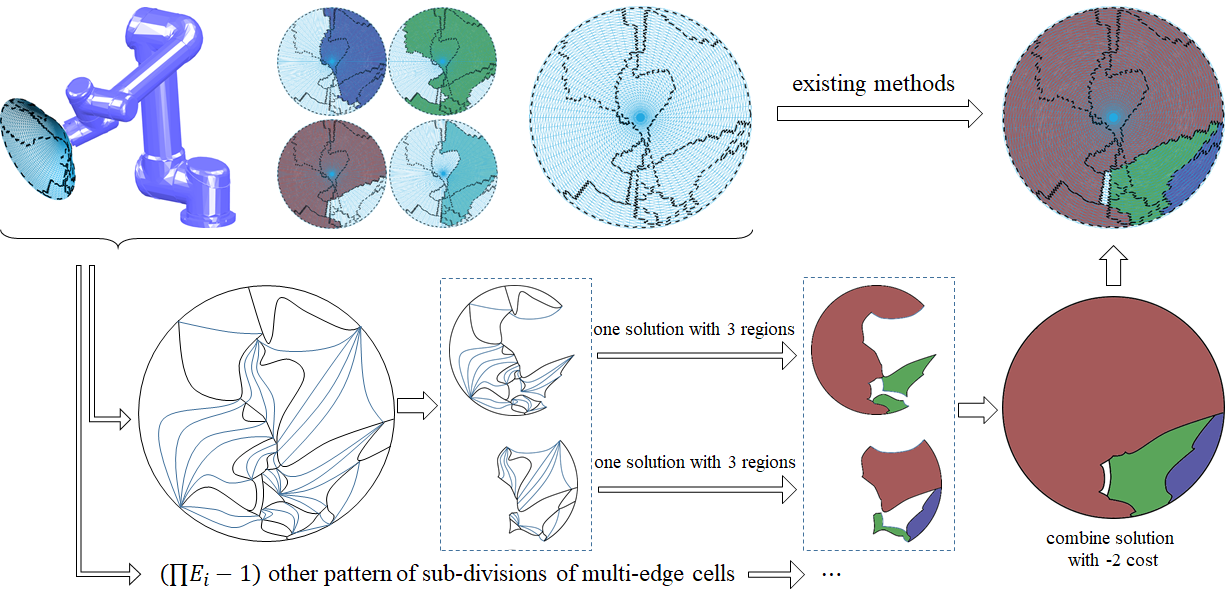
\includegraphics[width = 0.96\textwidth]{figures/hat_exp/fig_hat}
%\caption{\textcolor{blue}{What if I directly use the sub-graph in this experiment to be the demo figures of the above algorithm section? }}\label{fig:hat}
%\end{figure*}

\begin{comment}
% <ty> I commented out the figures. There are too many figures which may be difficult to layout. 
\begin{figure}[t]
\centering
\subfigure[]{
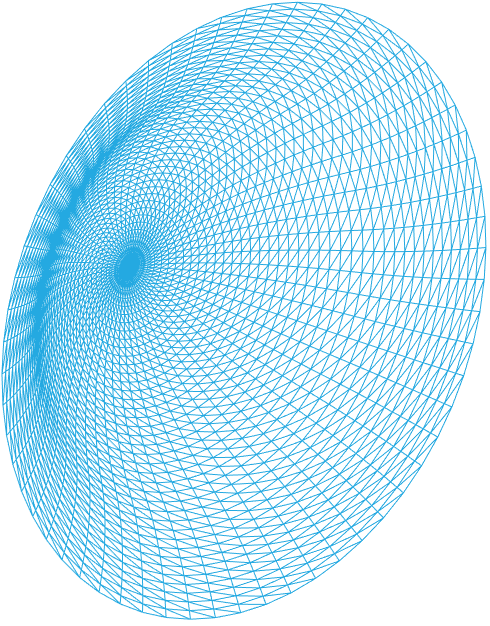
\includegraphics[width=0.18\textwidth]{figures/hat_exp/mesh}\label{fig:object:a}
}
\subfigure[]{
	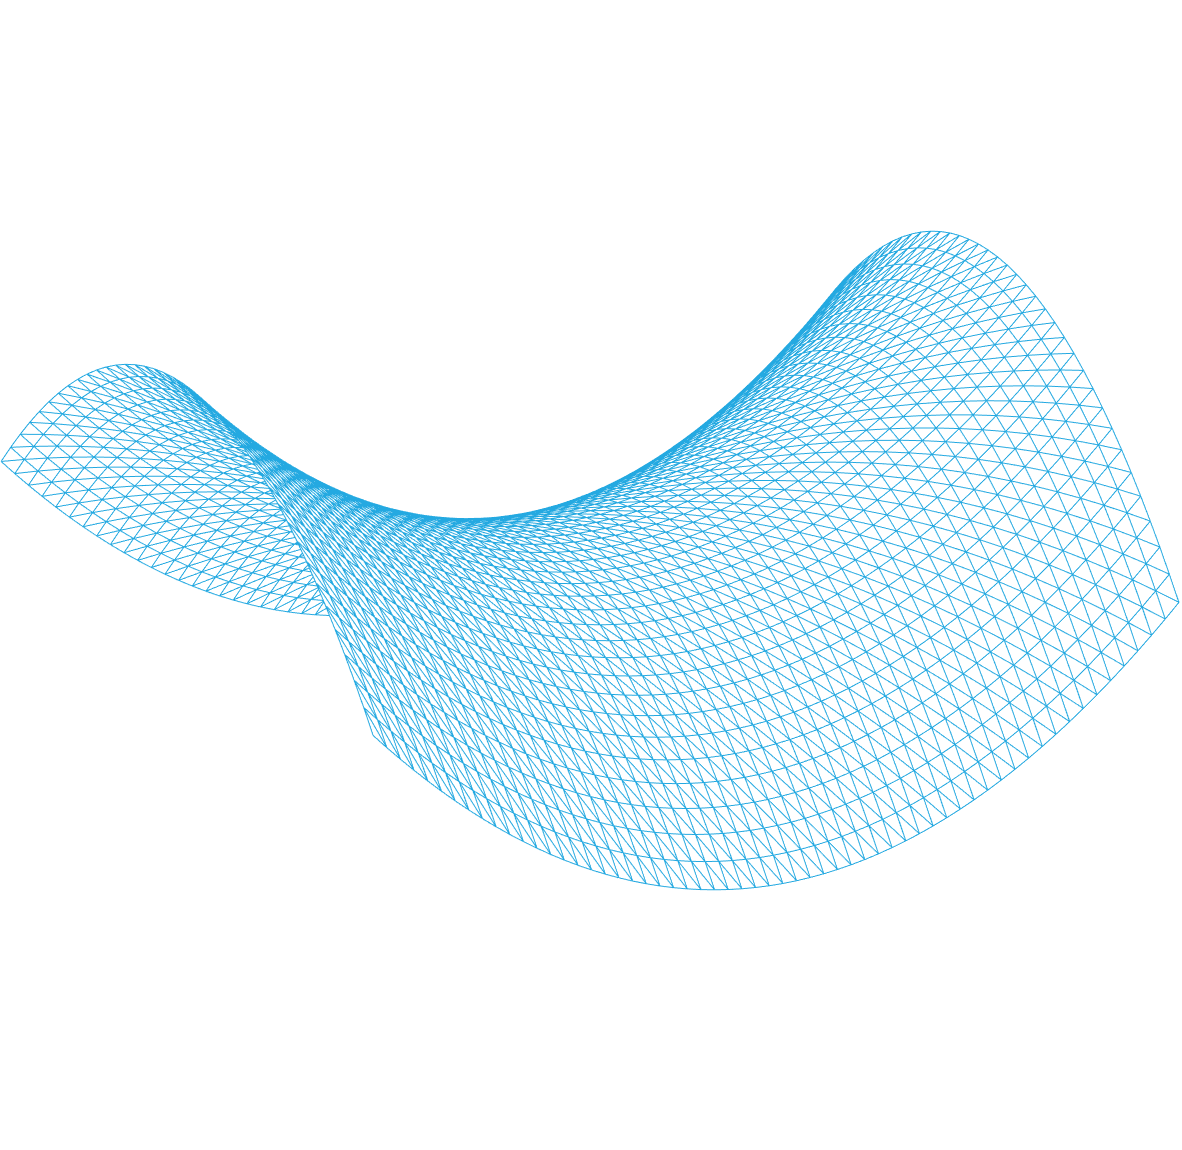
\includegraphics[width=0.18\textwidth]{figures/saddle_exp/mesh}\label{fig:object:b}
}
\subfigure[]{
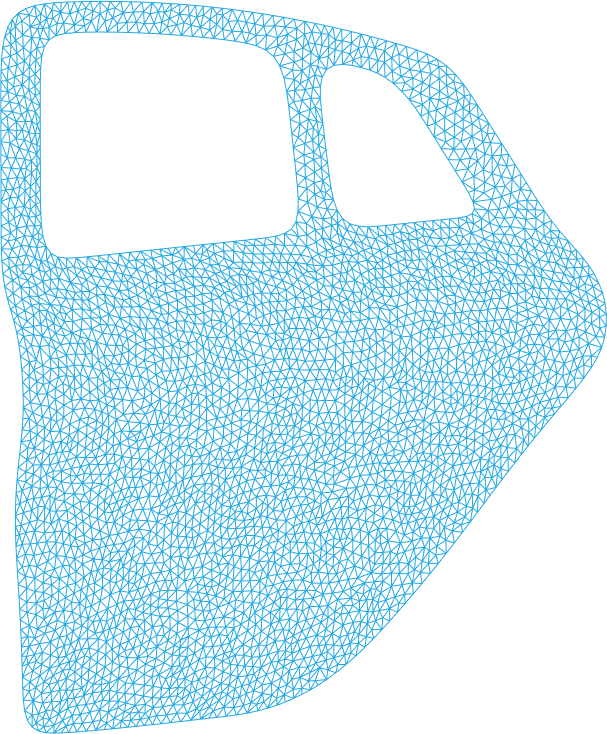
\includegraphics[width=0.18\textwidth]{figures/cardoor_exp/mesh}\label{fig:object:c}
}
\subfigure[]{
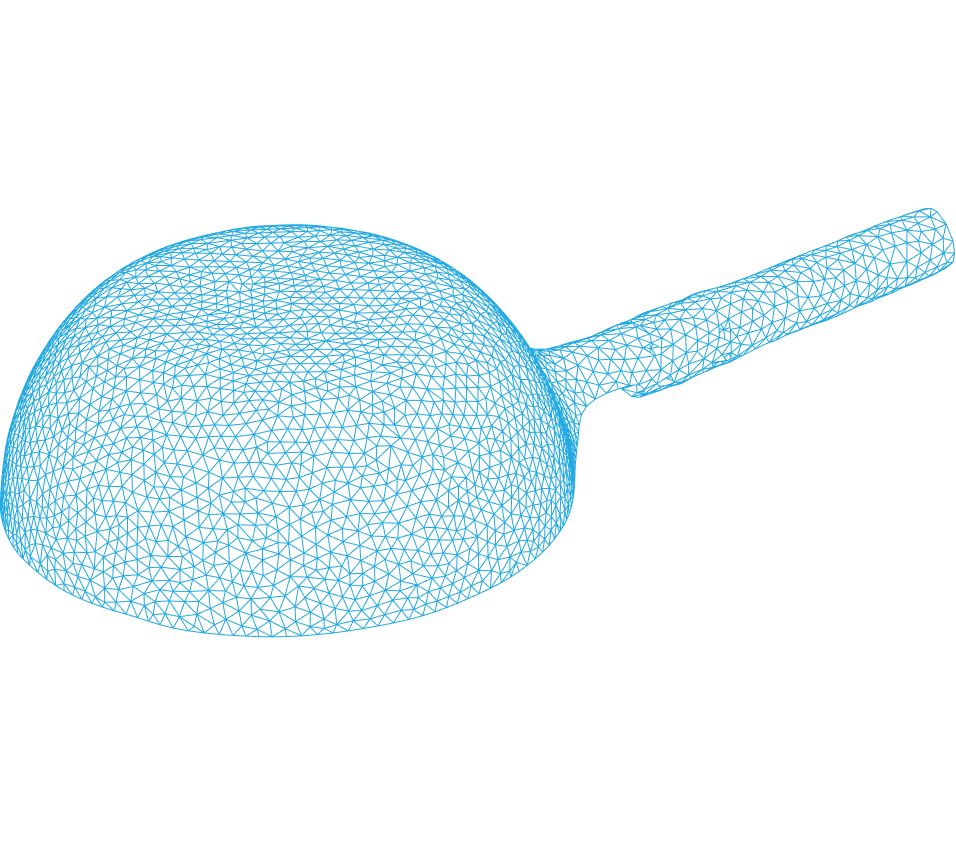
\includegraphics[width=0.18\textwidth]{figures/wok_exp/mesh}\label{fig:object:d}
}
\caption{The objects used to experimentally illustrate the results, Section~\ref{section_results}.}
\label{fig:object}
\end{figure}
\end{comment}

\begin{figure*}[t]
\centering
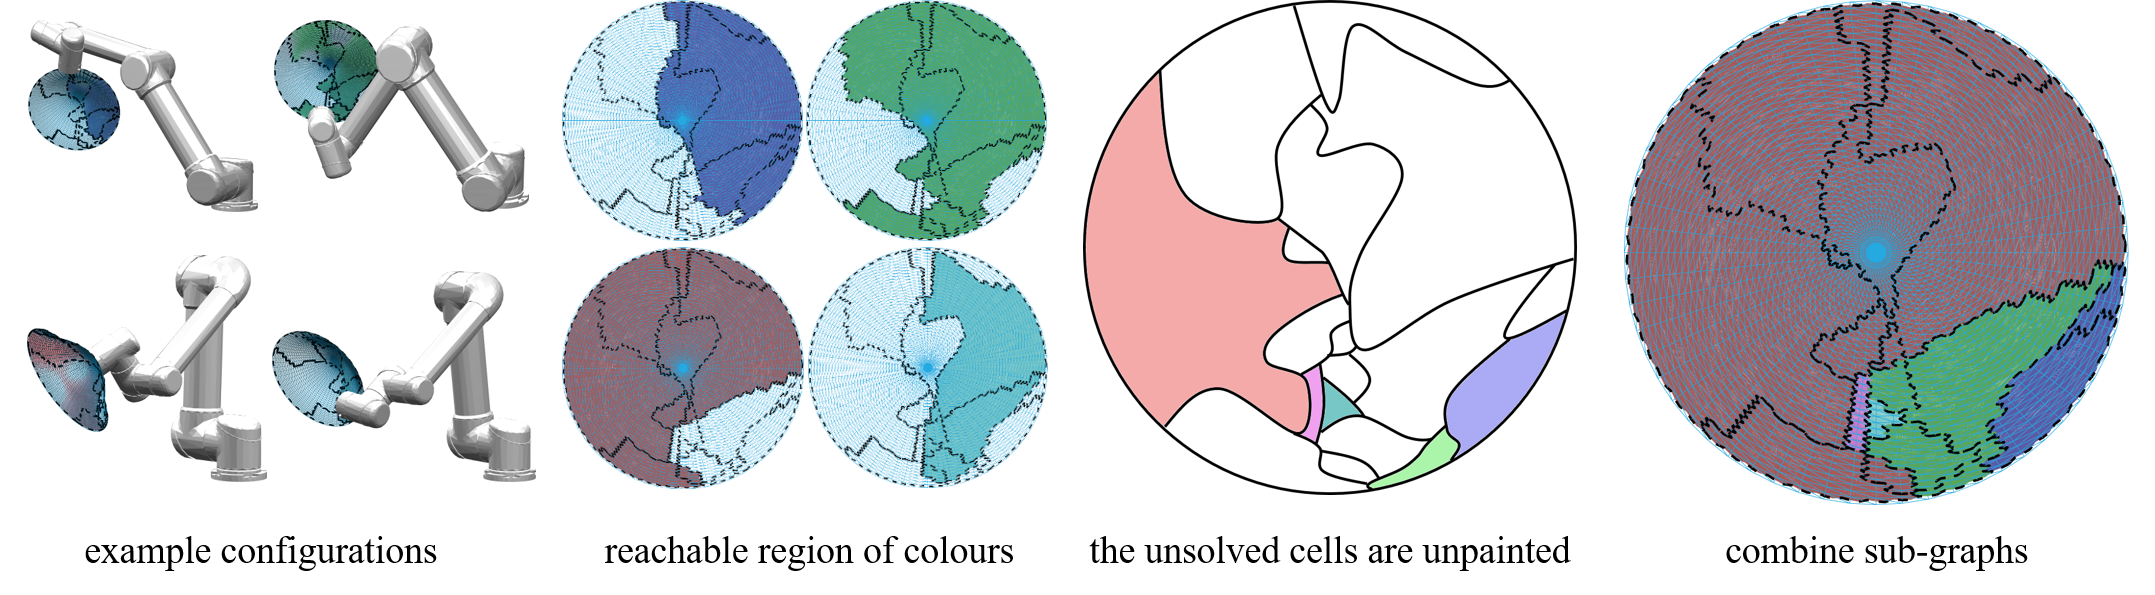
\includegraphics[width=0.96\textwidth]{figures/hat_exp/fig_hat_3}
\caption{The coverage task of a hat-shape object. The reachable area of different colours and one of their corresponding configurations are depicted. After painting all $1$-colour cells, the unsolved graph is %exactly the same one as we have discussed in Section \ref{section_graph_separation}. }
separated and solved as described in Section~\ref{section_graph_separation}, with the step-by-step process illustrated in Fig.~\ref{fig:steps}. } 
\label{fig:hat}
\end{figure*}
\begin{figure*}[t]
\centering
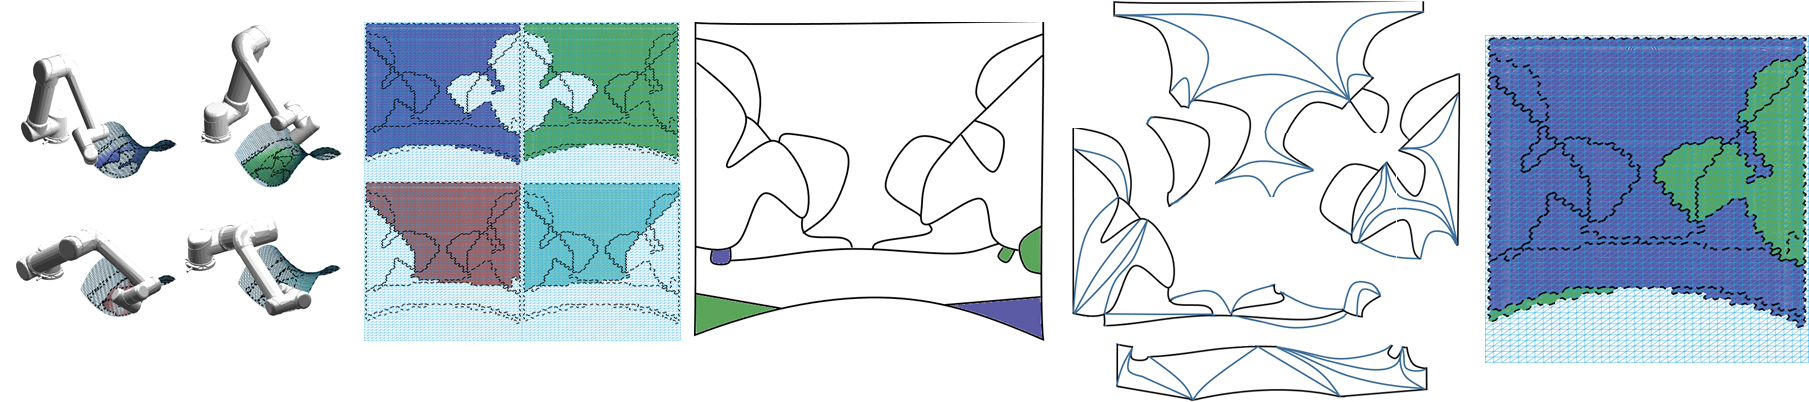
\includegraphics[width=0.96\textwidth]{figures/saddle_exp/comb_2}
\caption{The coverage task of a saddle surface. The reachable area of different colour and one of their corresponding configurations are depicted. After painting all $1$-colour cells, the unsolved graph is separated into $5$ sub-graphs. Finally, all optimal solutions can be collected with 2 end-effector lift-offs.}
\label{fig:saddle}
\end{figure*}


\begin{table*}
\centering
\caption{Experimental results}\label{table:results}
\begin{tabular}{  c | c | c | c | c | c | c | c  }
\hline
Object & Num. of Cells$^1$& Num. of Edges$^2$ & Algorithm & Lift-offs$^3$  &  Theoretical Bound$^3$ & Num. of Iterations$^4$ & Time$^5$ \\
\hline
\hline
\multirow{2}{*}{Hat-shaped (Fig.~\ref{fig:hat})} & \multirow{2}{*}{13(18)} & \multirow{2}{*}{35(51)} & \cite{Yang2020Cellular}  & $\mathbf{4}$ & $1.27*10^{28}$  & $4.50*10^7$ & 26.05s\\
\cline{4-8}
&&& Ours & $\mathbf{4}$ & $\mathbf{4.28*10^{14}}$ & $\mathbf{2.46*10^4}$ & \textbf{94ms}\\
\hline
\multirow{2}{*}{Saddle-shaped (Fig.~\ref{fig:saddle})} & \multirow{2}{*}{12(17)} & \multirow{2}{*}{37(48)} & \cite{Yang2020Cellular} & $\mathbf{2}$ & $2.86*10^{29}$ &  $8.71*10^8$ & 2.97h \\
\cline{4-8}
&&& Ours & $\mathbf{2}$ & $\mathbf{4.33*10^{16}}$ & $\mathbf{2.03*10^6}$ & \textbf{7.02s}\\
\hline
\multirow{2}{*}{Car Door-shaped (Fig.~\ref{fig:cardoor})} & \multirow{2}{*}{9(10)} & \multirow{2}{*}{16(35)} & \cite{Yang2020Cellular} & $\mathbf{1}$ & $2.32*10^{11}$ & $1.54*10^5$ & 48.94s\\
\cline{4-8}
 & && Ours & $\mathbf{1}$ & $\mathbf{3.46*10^3}$ & \textbf{405} & \textbf{125ms}\\
\hline
\multirow{2}{*}{Wok-shaped (Fig.~\ref{fig:wok})} &\multirow{2}{*}{9(15)}&\multirow{2}{*}{28(42)} & \cite{Yang2020Cellular} & $\mathbf{4}$ & $6.68*10^{13}$ & $1.24*10^4$ & 1.13s\\
\cline{4-8}
&&& Ours & $\mathbf{4}$ & $\mathbf{6.91*10^3}$ & \textbf{27} & $\mathbf{<}$\textbf{1ms}\\
\hline
\end{tabular}
\begin{tablenotes}
\item $^1$ Num. of Cells: Number of non-unique colour cells (number of all cells). 
\item $^2$ Num. of Edges: Number of internal edges (number of edges). 
\item $^3$ All results are optimal in the number of end-effector lift-offs, since both solvers are optimal. 
\item $^3$ The theoretical bounds are calculated based on a specific designing of cell sub-divisions. The sub-divisions for the hat-shaped object and the saddle-shaped object have been shown in Fig.~\ref{fig:hat} and Fig.~\ref{fig:saddle}, whilst the detailed illustrations for the car door-shaped object and the wok-shaped object are omitted. 
\item $^4$ One iteration corresponds to sub-dividing a cell or colouring the whole graph.  
\item $^5$ The computational time is measured on a PC computer with I7-8700 CPU, 11 threads in parallel. 
\end{tablenotes}
\end{table*}


\section{Experimental Results}\label{section_experiment}
\label{section_results}

The proposed solution is tested experimentally by simulating the NCPP with a non-redundant manipulator (6 DoF Universal Robot UR5) on four arbitrarily shaped objects, a hat-like concave semi-sphere, a saddle surface, a car door like surface, and a wok-like surface, as shown in Fig.~\ref{fig:hat}, Fig.~\ref{fig:saddle}, Fig.~\ref{fig:cardoor} and Fig.~\ref{fig:wok}.
In all experiments, only one side is considered. 
\begin{color}{blue}
The reader is referred to the supplemented video for the animation of the manipulator motion. 

A comparative analysis is provided to compare the performance of the proposed solver IMCGS against the existing enumerative solver in~\cite{Yang2020Cellular}. 
All experiments were implemented on a PC computer with I7-8700 CPU, 11 threads in parallel. 
For fair comparison, both solvers are executed subjected to the same standard tree pruning processes. 
All statistics have been detailed in Table.~\ref{table:results}.
Specif, 
\begin{enumerate}
\item When the number of painted colours for a partly-solved graph has been larger than the number of regions in the currently optimal solution, we remove this graph. 
\item Cells are reindexed in the edge-number-increasing order, so that cells with large number of edges (hence may generate enormous branches after its sub-division) are less likely to be enumerated. 
\item When a sub-cell is enforced to be connected to multiple adjacent cells, its possible colours can only be the intersecting set of the possible colours of all these adjacent cells. 
Specifically, the intersecting set of an arbitrary set with a single-element set is the single-element set itself, or the empty set (leading to the pruning of this enumerated case). 
Hence an adjacent cell with a unique colour will simplify the enumeration significantly. 
\item For two sub-cells gapped by a cutting path, when one colour is chosen by one sub-cell, it is eliminated from the set of possible colours of the other sub-cell.
\end{enumerate}
\end{color}

\subsection{Optimal NCPP on a Hat-shape Object}
An illustration of the solving process for the hat-shape object is depicted in Fig.~\ref{fig:hat}. 
Four continuous sets of manipulator configurations are represented in blue, red, green and cyan colour separately. $1$-colour cells have been directly drawn to the graph. 
%Using existing algorithms~\cite{Yang2020Cellular}, the initial topological graph is directly enumerated. We need to iteratively decide whether keep/remove each topological edges, and choose colour for each (sub-)cells, leading to complexity as (\ref{equ:tmech}). One of the graph after cell sub-divisions is shown in Fig.~\ref{fig:hat}.  
The cell sub-divisions correspond to the description provided earlier in Fig.~\ref{fig:complicated_graph}.
For the algorithmic complexity there are $43$ cells. The possible colours of each cell are known. As for edges, there are $44$ unsolved edges (drawn in black) and $30$ manually created edges - enforced to be kept (drawn in blue). Plus $9$ edges which are connected to unreachable area (a fifth colour), which need not solving. Using the naive enumeration~\cite{Yang2020Cellular} proposed in the literature, %~\cite{Yang2020Cellular} - we've repeated this too many times I feel
$35$ edges and all colours of all cells are enumerated, resulting in an algorithmic complexity described by 
\begin{equation}
{\color{red}2^{35}\times}
\begin{aligned}
&\overbrace{2\times2\times3\times2\times2\times2\times{\color{red}2\times2\times}}^{\textbf{all cells in sub-graph 1, shown in Fig.~\ref{fig:characteristic_string}}}\\
&2\times3\times3\times2\times2\times3\times2\times3\times2\times{\color{red}3\times}\\
&2\times2\times2\times2\times2\times2\times{\color{red}2\times}\\
&2\times3\times3\times4\times4\times{\color{red}3\times4\times}\\
&3\times3\times2\times3\times3\times4\times4\times{\color{red}3\times}\\
&3\times4\times3
\end{aligned}
\approx 1.27\times10^{28}
\end{equation}
% Please note there is a minor abuse of notation in the arrangement of the numbers above simply so that they can be easier to compared with the optimal solution below. 
%\begin{equation}
%2^{35}\cdot \underbrace{2\times 2\times \cdots \times 3}_{43 \mbox{ terms, number of colours}} \approx 1.2705*10^{28}
%\end{equation}
Using the proposed algorithm, the length of the boundary for each sub-graph is $6, 11, 9, 6, 10, 5$ respectively. The reader is referred to the sub-graph $1$ example
employed to discuss the process in detail in Sections~\ref{section_intersection} and~\ref{section_graph_separation}. Detail results for the other cases are ommited for lack of space, 
but follow the same process. 
The number of colours for the boundary cells in each sub-graph is included in the multiplicative factor, so the algorithm complexity derives in the multiplication of 
the complexity of all sub-graphs, given by 
\begin{equation}
\begin{aligned}
&\overbrace{2\times2\times3\times2\times2\times2\times}^{\textbf{internal cells shown in Fig.~\ref{fig:characteristic_string}}}\\
&2\times3\times3\times2\times2\times3\times2\times3\times2\times\\
&2\times2\times2\times2\times2\times2\times\\
&2\times3\times3\times4\times4\times\\
&3\times3\times2\times3\times3\times4\times4\times\\
&3\times4\times3
\end{aligned} \approx 4.28\times10^{14}
\end{equation}



\subsection{Optimal NCPP on a Saddle-shape Object}
Another example is provided with the analysis of the outer shell of a saddle-shape object. In this case the surface normal varies greatly as the end-effector moves 
along the surface, representing a challenging manipulator planning problem in adopting poses that would benefit the continuous coverage this paper is interested in. 
The algorithmic complexity given cell sub-divisions is shown in Fig.~\ref{fig:saddle}. For the naive enumeration case~\cite{Yang2020Cellular}, the overall complexity is given by 
%\begin{equation}
\begin{flalign}
&{\color{red}2^{37}*}~
\begin{aligned}
&2\times2\times2\times2\times2\times2\times2\times2\times2\times{\color{red}2\times}\\
&3\times2\times2\times2\times2\times2\times2\times \\
&~~~~3\times4\times4\times3\times2\times2\times2\times3\times{\color{red}3\times}\\
&3\times2\times2\times2\times2\times3\times3\times2\times{\color{red}2\times}\\
&4\times4\times4\times4\times4\times4\times3\times4\times{\color{red}4\times}\\
&3
\end{aligned}&\\
&\approx 2.86\times10^{29}&\nonumber
\end{flalign}
%\end{equation}
Applying the proposed algorithm, the complexity is reduced to
\begin{flalign}
&\begin{aligned}
&2\times2\times2\times2\times2\times2\times2\times2\times2\times\\
&3\times2\times2\times2\times2\times2\times2\times\\
&~~~~3\times4\times4\times3\times2\times2\times2\times3\times\\
&3\times2\times2\times2\times2\times3\times3\times2\times\\
&4\times4\times4\times4\times4\times4\times3\times4\times\\
&3
\end{aligned}
\approx 4.33\times10^{16}&
\end{flalign}
The overall results are gathered in Table~\ref{table:results} for easier comparison, collecting the substantial computational improvement in 
the number of edges for each problem ($35$ and $37$ repectively). As the geometry of the object of interest becomes more intricate, 
the benefit of the proposed scheme to be able to find paths with minimal discontinuities in joint-space with a reduced computational effort 
becomes also more apparent.

\begin{figure}[t]
\centering
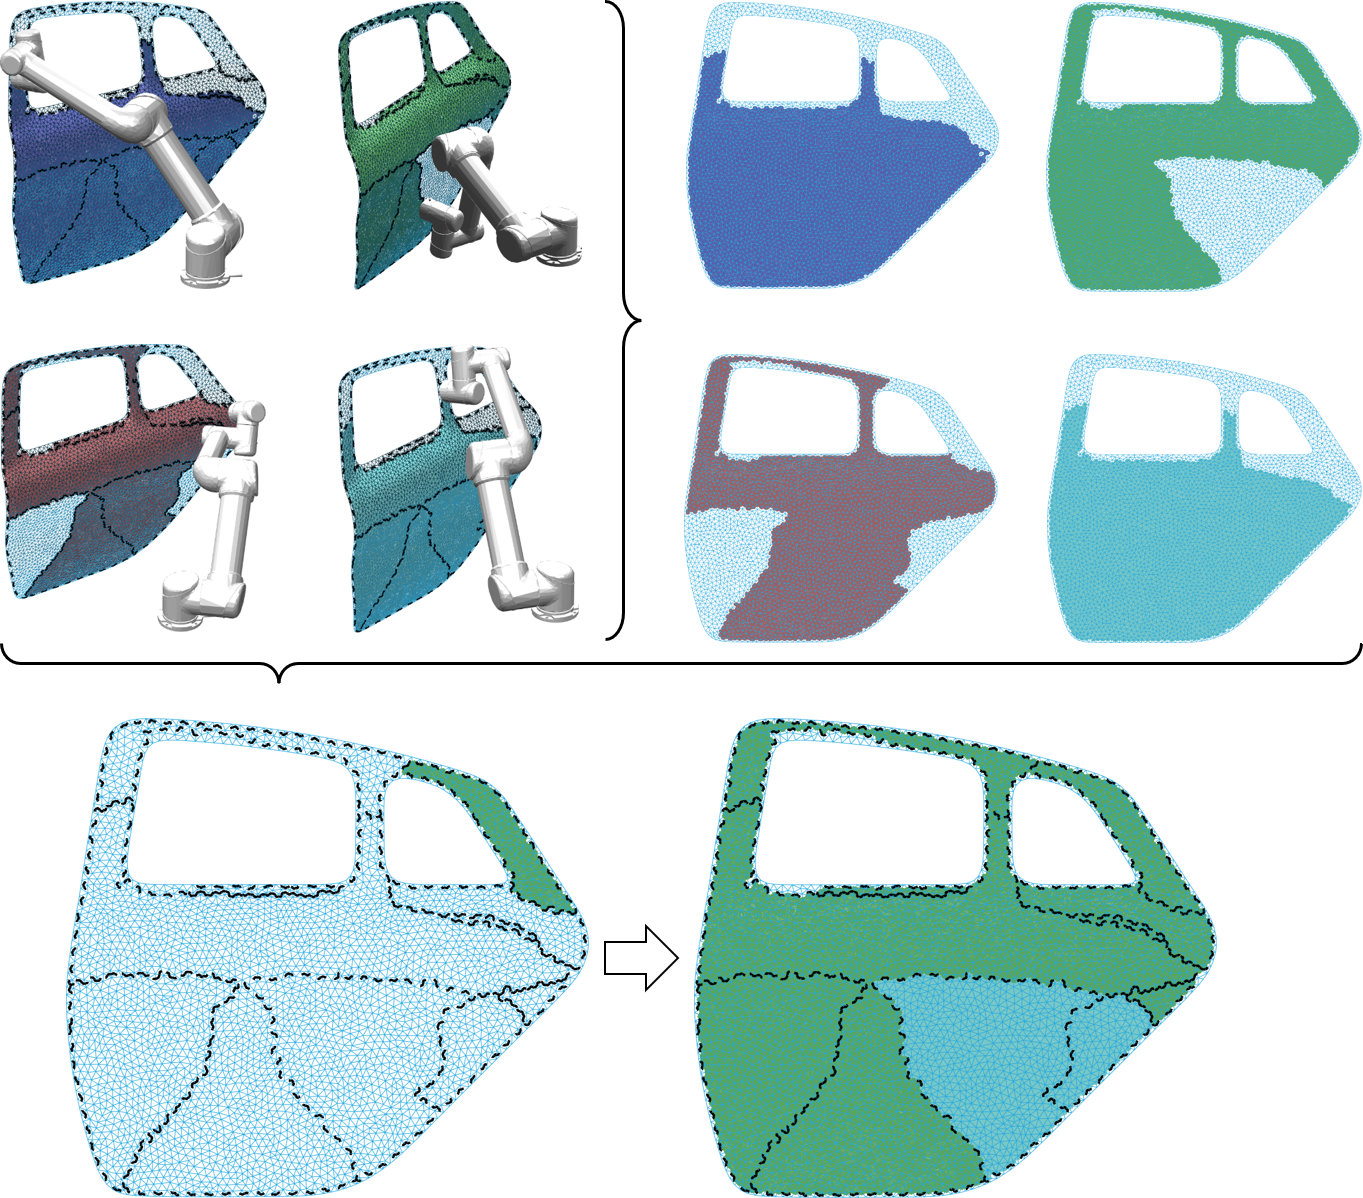
\includegraphics[width=0.48\textwidth]{figures/cardoor_exp/cardoor_comb}
\caption{\textcolor{blue}{Car door example. 
Single-colour cells have been directly drawn to
the initial graph. }}\label{fig:cardoor}
\end{figure}

\begin{figure}[t]
\centering
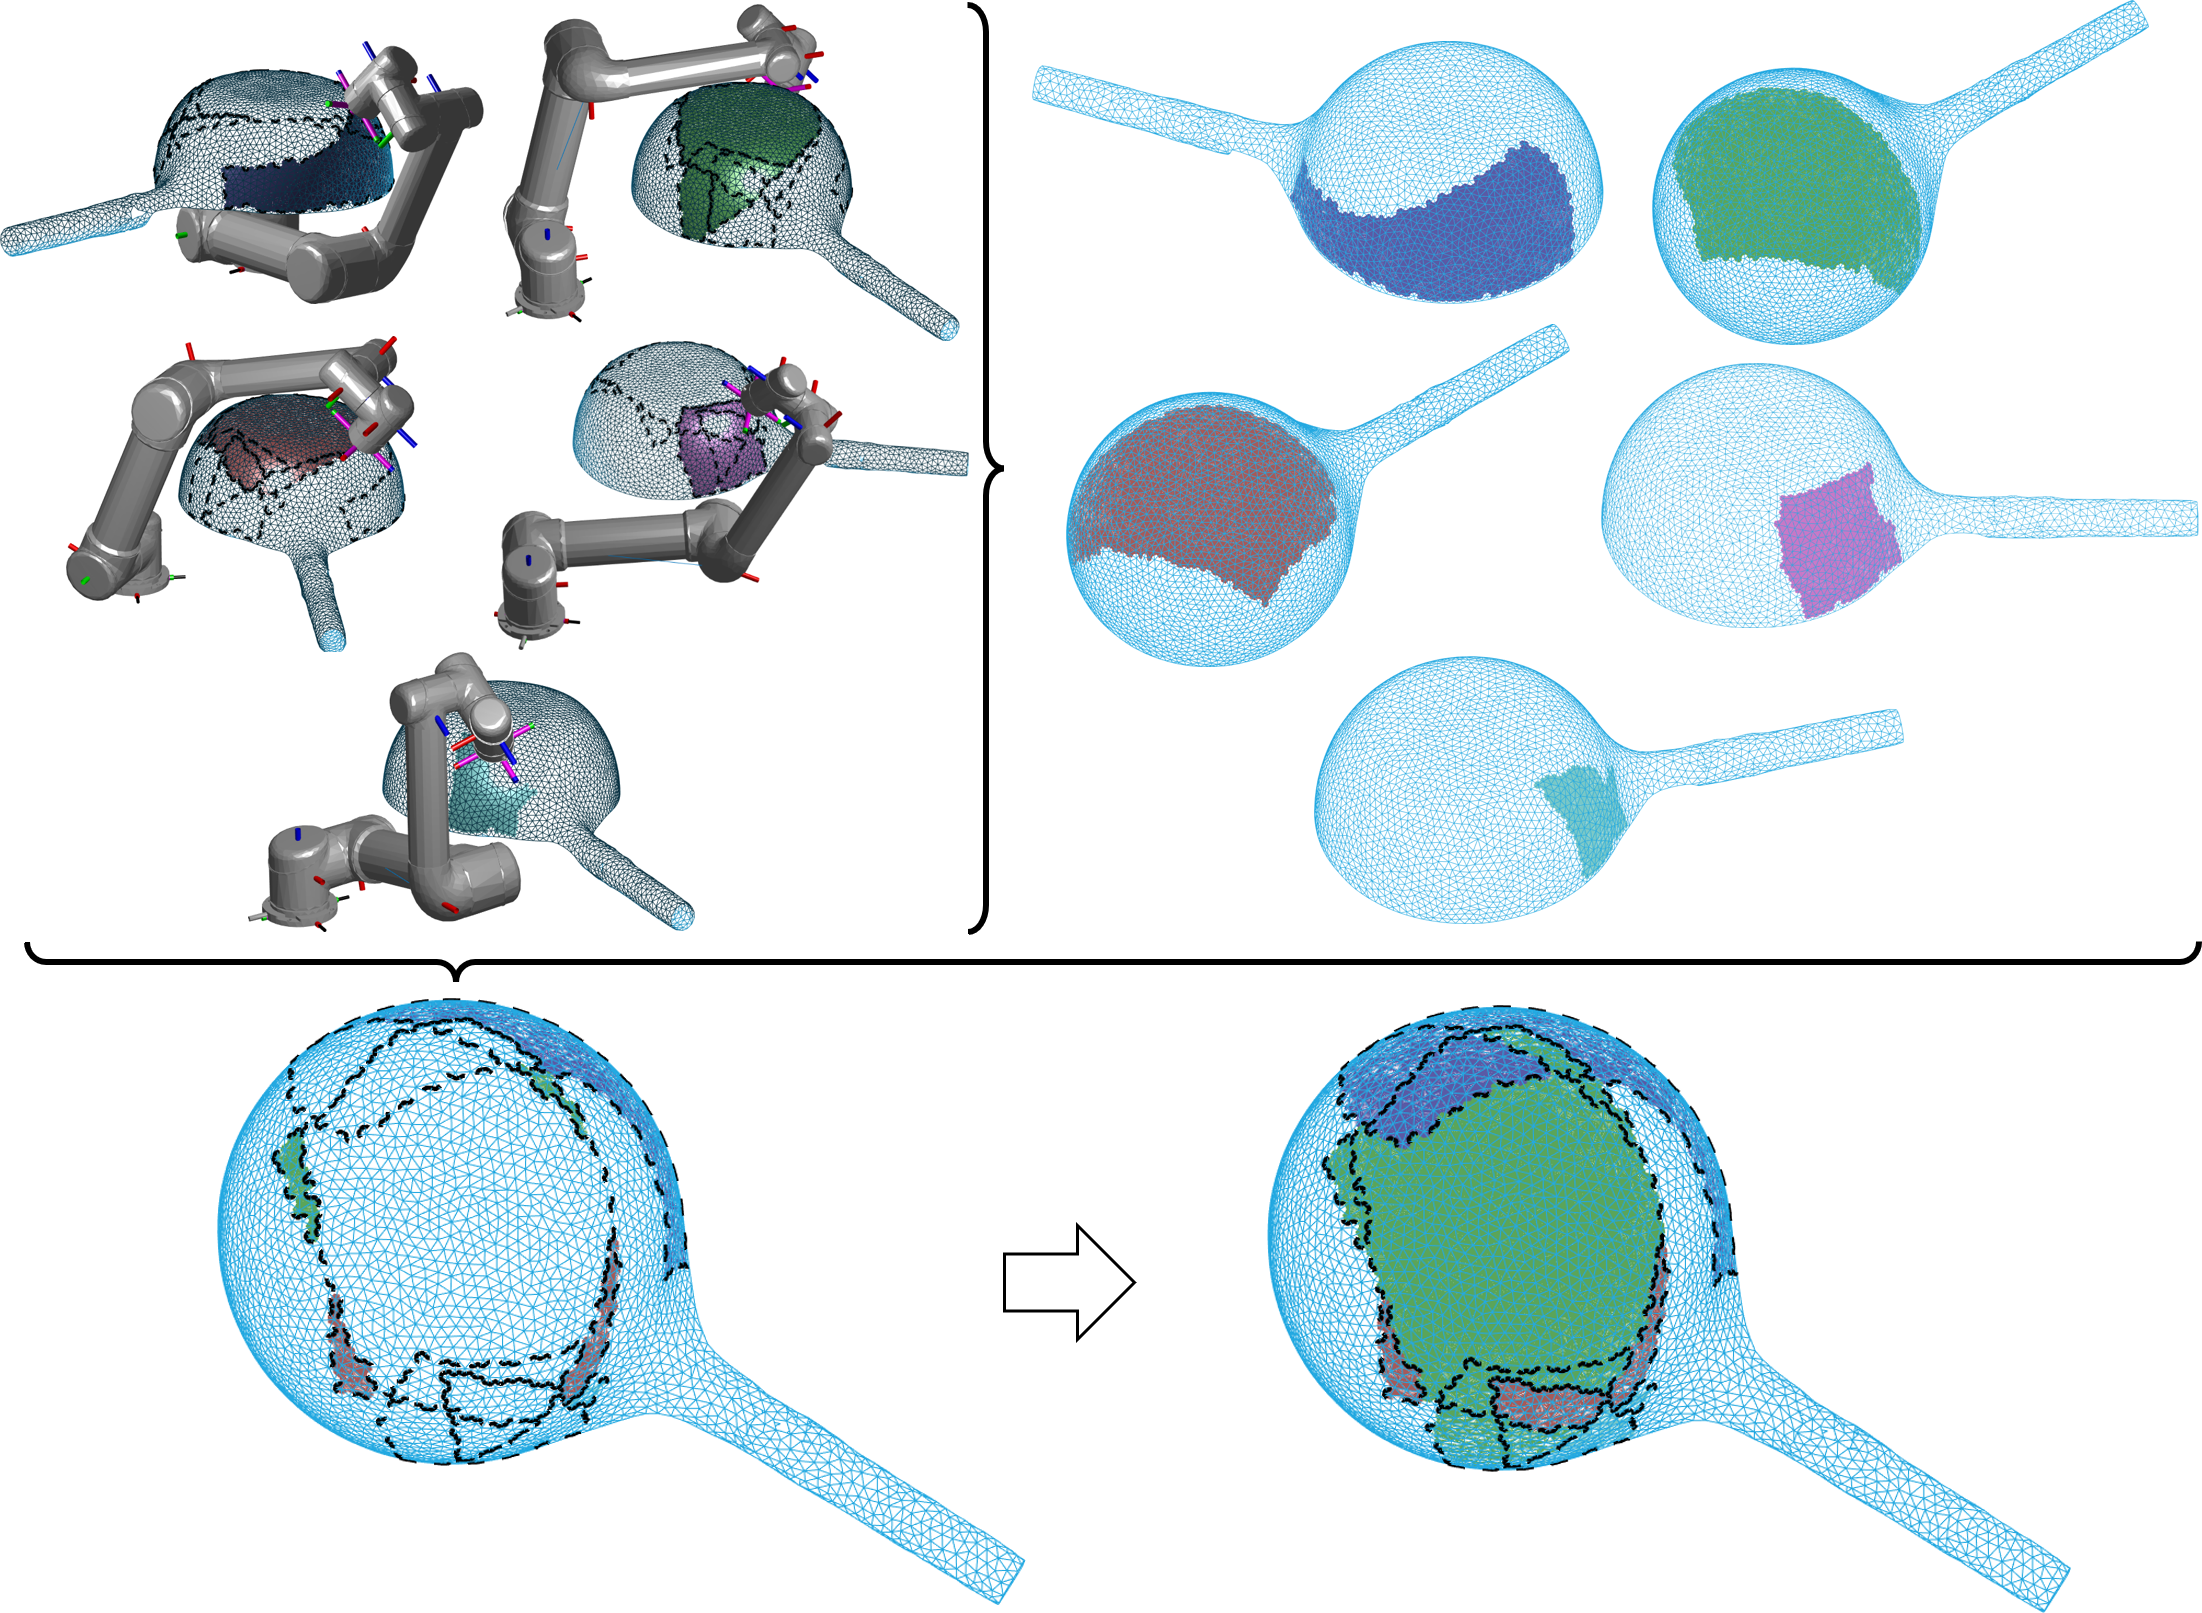
\includegraphics[width=0.48\textwidth]{figures/wok_exp/wok_comb}
\caption{\textcolor{blue}{Wok example. 
Single-colour cells have been directly drawn to
the initial graph. 
}}\label{fig:wok}
\end{figure}

\begin{color}{blue}
\subsection{Further Evaluations}
Further simulation tests are shown in Fig.~\ref{fig:cardoor} and Fig.~\ref{fig:wok}. 
The object surfaces are now unstructured meshes, where the proposed solver is still applicable. 

In the former test, a car door mesh is considered. 
Among the $10$ cells in this graph, one cell (referred to as Cell $1$ in this experiment) has $16$ edges, whilst all other cells have no more than $4$ adjacent connectable cells. 
Recalling that cells with $\leq 3$ edges need not be sub-divided, and the number of sub-divisions for a $4$-edge cell can be easily verified as $2$ (the diagonals of the topological quadrangle). 
Hence, enumerating Cell $1$ consumes the largest proportion of computational time for the solver. 
As indicated before, Cell $1$ has the largest number of edges, so it is the last cell to be enumerated. 
In contrast to the existing solver, the proposed improved solver does not enumerate edges nor possible colours of cells, hence creates a significant smaller number of enumerated cases that requires the enumeration of Cell $1$. 
Result shows that the computational time of the improved solver IMCGS (125ms) is much more efficient than the state-of-the-art method (48.94s). 

In the latter, a wok-like mesh is tested. 
For simplicity in this example, the handle of the wok is not considered part of the mesh for coverage, and it is set as an obstacle. 
To form a more challenging set of valid configurations, we assume that the wok floats in the air without support, so the manipulator can perform the coverage motion with its forearm below the wok. 
Although there are $15$ cells in the graph, $6$ of them only have a unique colour (painted in the initial graph in Fig.~\ref{fig:wok}), which give birth to a much more efficient tree pruning processes (see the huge reduction of the number of iterations against the theoretical bound). 
Finally, the proposed solver is able to solve the graph within 1ms. 

\end{color}

\section{Conclusions}
An advancement to efficiently solve non-repetitive coverage tasks with a non-redundant manipulator is proposed in this work. 
The core concept is the introduction of intersection-free sub-graphs, which permit the separation of a graph 
into sub-graphs at the points where the multiplicity of optimal solutions originate. 
The implicit enumeration when the sub-graphs are recombined in search of the full solution derives in a mathematically proven exponential improvement in the order of $2^N$, $N$ representing the number of topological edges in the graph. 
This is particularly relevant for intricate task-space graphs, where an exhaustive search for solutions with all the cells and edges is unattainable. 
\textcolor{blue}{The proposed graph solver, called IMCGS, has been supplemented by a detailed video and an open source implementation in C++ for the benefit of the research community.}
Comprehensive experimental results with step-by-step derivations to illustrate the proposed algorithm are supplied that demonstrate the validity of the novel scheme. 
\label{section_conclusion}


%% Use plainnat to work nicely with natbib. 

%\newpage 

% Added preliminaries as appendix
%\begin{appendices}
\begin{color}{blue}
\section*{Appendix: Glossary}
\begin{enumerate}
\item Colour: A continuous set of collision-free, non-singular manipulator configurations with the end-effector staying on the task-space surface. 
\item Cell: A part of task-space reachable region, where all points having the same set of possible colours. 
\item Edge: The common boundary between two cells. 
\item Graph: The combination of cells and edges. 
\item Cutting Path: A task-space curve that enforces its two sides cannot be painted the same colour. 
\item Cell Sub-division: Dividing the region of a cell into multiple sub-parts by cutting paths. 
\item Graph Solution: An assignment for each cell a colour within its set of possible colours. 
\item Cost: Grouping the same-colour adjacent cells in one group, the cost is the number of groups, visualised as the number of connected painted regions. 
\item Optimal Solution: The graph solution with minimum cost. 
\item Sub-graph: a connected subset of cells, together with all edges that connect them. 
\item Boundary of Sub-graph: A closed chain of the edges that connect a cell inside the sub-graph and a cell outside the graph. \item Boundary Cell: The cells in a sub-graph which are adjacent to cells outside this sub-graph. 
\item Internal Cell: The non-boundary cells in a sub-graph. 
\item Intersection-free Sub-graph: A sub-graph with all its boundary cells having a unique colour, such that the number of optimal solution of the sub-graph is unique. 
\item Strip: A kind of sub-graph that is intersection-free given any possible colours of its boundary cells.
\end{enumerate}

\end{color}

%\end{appendices}

\bibliographystyle{ieeetr}
\bibliography{tro21}

\end{document}


